\documentclass{article}

% NeurIPS 2026 Evaluations & Datasets Track (single-blind)
\usepackage[eandd, nonanonymous]{neurips_2026}

\usepackage[utf8]{inputenc}
\usepackage[T1]{fontenc}
\usepackage{hyperref}
\usepackage{url}
\usepackage{booktabs}
\usepackage{amsfonts}
\usepackage{amsmath}
\usepackage{amssymb}
\usepackage{amsthm}
\usepackage{nicefrac}
\usepackage{xcolor}
\usepackage{enumitem}
\usepackage{mathtools}
\usepackage{graphicx}
\usepackage[normalem]{ulem}
\usepackage{tikz}
\usetikzlibrary{positioning, arrows.meta, fit, backgrounds}

% =====================================================================
% Design system: 5-color palette shared with generate_figures.py
% =====================================================================
\definecolor{defabBlue}{HTML}{1F3A6B}
\definecolor{defabTeal}{HTML}{3D6B7A}
\definecolor{defabGold}{HTML}{D9A441}
\definecolor{defabRed}{HTML}{B0413E}
\definecolor{defabGray}{HTML}{6B7280}

% Theorem environments
\newtheorem{theorem}{Theorem}[section]
\newtheorem{proposition}[theorem]{Proposition}
\newtheorem{corollary}[theorem]{Corollary}
\theoremstyle{definition}
\newtheorem{definition}[theorem]{Definition}
\newtheorem{example}[theorem]{Example}
\newtheorem{remark}[theorem]{Remark}

% Custom commands
\newcommand{\D}{\mathcal{D}}
\newcommand{\Dm}{\mathcal{D}^{-}}
\newcommand{\Dfull}{\mathcal{D}^{\mathrm{full}}}
\newcommand{\HB}{\mathcal{H}_B}
\newcommand{\Hcand}{\mathcal{H}_{\mathrm{cand}}}
\newcommand{\Hgold}{\mathcal{H}^{*}}
\newcommand{\Rgold}{\mathcal{H}^{*}_3}
\newcommand{\Rs}{R_s}
\newcommand{\Rd}{R_d}
\newcommand{\Rdf}{R_{df}}
\newcommand{\partfunc}{\kappa}
\newcommand{\Supp}{\mathrm{Supp}}
\newcommand{\Crit}{\mathrm{Crit}}
\newcommand{\CritStar}{\mathrm{Crit}^{*}}
\newcommand{\Exp}{\mathrm{Exp}}
\newcommand{\Nov}{\mathrm{Nov}}
\newcommand{\Score}{\mathrm{Score}}
\newcommand{\proves}{\vdash}
\newcommand{\pDelta}{\vdash_{\Delta}}
\newcommand{\pPartial}{\vdash_{\partial}}
\newcommand{\defto}{\Rightarrow}
\newcommand{\strictto}{\rightarrow}
\newcommand{\defeatto}{\leadsto}
\newcommand{\comp}[1]{\overline{#1}}


\title{DeFAb: A Defeasible Abduction Benchmark and Verifier-Backed Finetuning Substrate for Foundation Models}

\author{%
  Patrick Cooper \\
  Department of Computer Science\\
  University of Colorado Boulder\\
  Boulder, CO 80309 \\
  \texttt{patrick.cooper@colorado.edu} \\
}


\begin{document}

\maketitle


\begin{abstract}
A rule-based logic solver resolves every instance in our benchmark in under 50 microseconds with 100\% accuracy. The best frontier language model achieves 65\% at best, and drops to 7.8\% under rendering-robust evaluation. This gap is structural, not computational. We introduce \textsc{DeFAb} (\textbf{De}feasible \textbf{A}bduction \textbf{B}enchmark), a dataset, generation pipeline, and verifier-backed finetuning substrate that converts four decades of publicly funded knowledge bases into formally grounded evaluation instances for defeasible abduction: the task of constructing hypotheses that explain anomalies by overriding default conclusions while preserving unrelated expectations. The pipeline pairs taxonomic hierarchies (OpenCyc, YAGO, Wikidata) with behavioral property graphs (ConceptNet, UMLS) to produce 372,648+ instances across 33.75 million materialized rules from 18 knowledge sources, stratified into three difficulty levels with polynomial-time verifiable gold-standard hypotheses. Evaluation of four frontier models reveals a cascade of structural failures: two of four models score below random chance (16.7\%) on the rendering-robust metric; the best model achieves only 0.8\% at Level~3 under direct prompting; 80.9\% of Kimi-K2.5 responses fail to decode at all; and chain-of-thought prompting actively harms instruction-tuned models ($-14$~pp) while helping reasoning-optimized models ($+79$~pp). These findings reveal not underperformance but structural absence of defeasible reasoning capability. Beyond evaluation, the benchmark's polynomial-time verifier doubles as an \emph{exact reward function} for preference optimization: graded scoring directly yields DPO preference pairs, RLVR/GRPO rewards, and verifier-gated re-prompt signals, making DeFAb a self-contained finetuning substrate without reward model approximation. The dataset, generation pipeline, and evaluation harness are released under the MIT license at \url{https://huggingface.co/datasets/PatrickAllenCooper/DeFAb}.
\end{abstract}


%% ====================================================================
\section{Introduction}\label{sec:intro}
%% ====================================================================

A rule-based Answer Set Programming solver, running the same defeasible reasoning algorithm we use to generate our benchmark, resolves every evaluation instance with 100\% accuracy in under 50 microseconds~\cite{maher2001propositional}. The best frontier language model, under optimal chain-of-thought prompting, achieves 65\%. Under the rendering-robust metric --- the worst-case accuracy across four surface presentations of the same logical content --- it achieves 23.5\%, and two of four evaluated models score at or below random chance (16.7\% for six-choice selection). This gap is not a matter of scale or compute, but of what capability the models possess rather than what they are given.

The gap reflects three entangled structural deficits in current foundation models. The first is a deficit of \emph{grounding}: models lack an explicit epistemic structure distinguishing strict knowledge from revisable defaults, and cannot trace predictions to their supporting evidence~\cite{dunker2001intrinsically}. The second is a deficit of \emph{novelty}: without knowing which beliefs are revisable, models cannot identify where creative exceptions might apply. A striking biological illustration is the discovery of intrinsically disordered proteins (IDPs), proteins that lack fixed three-dimensional structure yet remain functionally essential. An AI trained on the prevailing structure-function dogma would be unlikely to hypothesize the existence of IDPs, because the hypothesis directly contradicts the domain knowledge encoded in its training corpus. The third deficit is one of \emph{belief revision}: even when models do update knowledge, they lack the formal machinery to ensure that updates respect the principle of minimal change~\cite{alchourron1985logic}, accommodating new evidence while disturbing as few existing commitments as possible. The IDP example illustrates all three deficits simultaneously, since the discovery requires not merely asserting that disordered proteins exist but doing so via a targeted revision that overrides the structure-function default for a specific subclass while preserving predictions about conventionally structured proteins.

Defeasible reasoning provides the structure these deficits demand. In a defeasible theory, every conclusion is derived through a traceable chain of strict and defeasible rules, every default is explicitly revisable, and every piece of evidence participates in an identifiable support set. This furnishes grounding, the machinery for novelty, and a concrete operationalization of rational belief revision through our conservativity requirement (Definition~\ref{def:conserv}), which ensures that resolutions preserve all expectations except the targeted anomaly and directly implements the AGM minimal-change postulate~\cite{gardenfors1988knowledge, katsuno1991propositional}.

The infrastructure to instantiate this framework at scale already exists, and it has existed for decades. Beginning in the early 1980s, large publicly funded programs --- Japan's Fifth Generation Computer Systems project~\cite{fuchi1984aiming, feigenbaum1993fgcs}, the United Kingdom's Alvey Programme~\cite{alvey1985ikbs}, the European ESPRIT initiative, and the United States DARPA Strategic Computing initiative that funded Cyc~\cite{lenat1990cyc, lenat1995cyc} --- pursued a research thrust whose explicit goal was the formal encoding of commonsense and expert knowledge in revisable logical form. This thrust continued through subsequent NSF-funded resources (WordNet~\cite{miller1995wordnet}, ConceptNet~\cite{speer2017conceptnet}), NIH biomedical infrastructure (UMLS~\cite{lindberg1993umls}, Gene Ontology~\cite{ashburner2000go}), EU-funded ontologies (LKIF Core~\cite{lkif2007}, BabelNet~\cite{navigli2012babelnet}), and the encyclopedic projects Wikidata~\cite{vrandecic2014wikidata}, DBpedia~\cite{lehmann2015dbpedia}, and YAGO~\cite{suchanek2024yago}. Together these efforts constitute one of the largest sustained investments in formally structured human knowledge ever undertaken, and they encoded by design exactly the two ingredients required for defeasible reasoning: default generalizations (taxonomic hierarchies, capability assertions, GCI axioms) and structured exceptions (Wikidata's P2303 ``exception to constraint'' property, ConceptNet's \texttt{NotCapableOf} edges, the Gene Ontology's \texttt{NOT}-qualified annotations). In the deep-learning era this infrastructure has been largely set aside, retained as an evaluation backdrop or a knowledge-graph completion source rather than as the active formal scaffold it was built to be. The contemporary failure modes of foundation models --- hallucination, the inability to revise defaults, the inability to localize a counterexample to a specific lemma --- are precisely the failure modes that the original government-funded programs aimed to prevent through formal structure. DeFAb takes the position that this infrastructure is not obsolete but underused, and that activating it as a verifier-backed substrate for both evaluation and training constitutes a renewed and principled thrust for AI progress: not a return to symbolic AI in opposition to learned methods, but a synthesis in which decades of formally structured public knowledge become the ground truth that makes verifier-grounded learning of defeasible reasoning possible.

A further obstacle threatens the construction of any benchmark in this space. For well-documented defaults and exceptions such as ``birds fly'' and ``penguins do not fly,'' we cannot distinguish genuine defeasible reasoning from the retrieval of memorized pretraining solutions. \citet{zhang2024gsm1k} demonstrated accuracy drops attributable to contamination on grade-school mathematics, and LiveCodeBench~\cite{jain2025livecodebench} exposed contamination even in frontier models through time-segmented evaluation. For defeasible reasoning benchmarks grounded in well-known knowledge bases, the risk is acute, and addressing it requires evaluation instances whose solutions provably fall outside any pretraining corpus.

We introduce \textsc{DeFAb} (\textbf{De}feasible \textbf{A}bduction \textbf{B}enchmark) to address these deficits jointly. Our contributions are sixfold. First, we provide a dataset and generation pipeline that converts definite logic programs into defeasible theories via a parameterized partition function $\partfunc$, with polynomial-time instance generation at three difficulty levels --- fact completion (Level~1), rule abduction (Level~2), and defeater abduction (Level~3) --- under formal conservativity guarantees (Corollary~\ref{cor:cubic}). Second, we develop a cross-ontology knowledge base extraction methodology that spans 18 knowledge sources and 33.75 million materialized rules drawn from four decades of publicly funded knowledge engineering, ranging from Cyc (1984) to UMLS 2025AB. Third, we introduce a synthetic contamination control that generates structurally isomorphic theories with invented predicate names verified for zero occurrence in Common Crawl via \texttt{infini-gram}~\cite{liu2024infini}, providing a per-model upper bound on contamination-attributable performance inflation. Fourth, our baseline evaluation of four frontier models reveals a cascade of structural failures: rendering-robust accuracy between 7.8\% and 23.5\% (with two models at or below random chance), Level~3 direct-prompting accuracy between 0.8\% and 23.6\%, an 80.9\% decoder failure rate for the weakest model, and a universal narrative-modality collapse of 55--70 percentage points. Fifth, a multimodal visual grounding modality (M5) extends the protocol to vision-language models by replacing or supplementing textual entity identification with images harvested from Wikidata~P18, VisualSem, and BabelNet. Finally, the same polynomial-time verifier that scores evaluation instances doubles as an \emph{exact} reward function for preference optimization, yielding margin-weighted DPO pairs, RLVR/GRPO rollout rewards, and verifier-gated re-prompt feedback for LLM-as-commander policies in the RTS game-grounded track --- without reward-model approximation.

The remainder of the paper is organized as follows. Section~\ref{sec:related} reviews related work. Section~\ref{sec:design} formalizes the generation pipeline, and Section~\ref{sec:sources} describes the source knowledge bases. Section~\ref{sec:example} presents a complete worked example. Section~\ref{sec:evaluation} reports the baseline evaluation, leading with the most informative failures. Section~\ref{sec:finetuning} develops the finetuning substrate, and Section~\ref{sec:discussion} discusses limitations and the pre-registered \textsc{DeFAb-Hard} difficulty hardening.


%% ====================================================================
\section{Related Work}\label{sec:related}
%% ====================================================================

Non-monotonic reasoning has a long formal history. Reiter's default logic~\cite{reiter1980logic} and McCarthy's circumscription~\cite{mccarthy1980circumscription} addressed the inadequacy of classical logic for commonsense reasoning, and Nute's defeasible logic~\cite{nute1987defeasible, nute1994defeasible} offered a computationally tractable alternative. The KLM framework~\cite{kraus1990nonmonotonic} provided axiomatic foundations for rational non-monotonic inference. The proof theory we adopt follows \citet{antoniou2001defeasible}, who together with \citet{maher2001propositional} established that propositional defeasible derivation has linear-time complexity --- a result that underlies the tractability of our generation pipeline. On the belief-revision side, the AGM postulates~\cite{alchourron1985logic, gardenfors1988knowledge} provide rationality conditions for updating beliefs under new evidence, with \citet{dalal1988investigations} introducing distance-based revision. Our conservativity requirement operationalizes minimal change in the defeasible setting, and our revision distance provides a tractable analogue of Dalal's distance metric.

Existing reasoning benchmarks largely evaluate forward, monotonic inference. ProofWriter~\cite{tafjord2021proofwriter} and LogicNLI~\cite{tian2021diagnosing} test deductive verification, not hypothesis generation; INABHYD~\cite{inabhyd2025} shows that language models fail to follow Occam's Razor in abductive contexts; and LogiDynamics~\cite{zheng2025logidynamics} studies the interplay of inductive, abductive, and deductive inference but over generic analogical tasks rather than formally specified defeasible theories. The closest related work is \textsc{DeFReasing}~\cite{allaway2025defreasing}, which probes defeasible property inheritance. DeFAb differs from \textsc{DeFReasing} in three fundamental ways: it is a construction task in which the model must generate the exception rule rather than classify given new information, it uses formally specified theories with verifier-backed gold standards computable in polynomial time, and its conservativity check operationalizes AGM minimal change in a way that classification-style benchmarks cannot.

The knowledge bases on which DeFAb is built reflect four decades of publicly funded investment in formal knowledge engineering. The 1980s produced large-scale systems from government AI programs --- Japan's FGCS project~\cite{fuchi1984aiming, feigenbaum1993fgcs}, the UK's Alvey Programme~\cite{alvey1985ikbs}, and Cyc~\cite{lenat1990cyc, lenat1995cyc} --- and this tradition continued through NSF-funded resources such as WordNet~\cite{miller1995wordnet} and ConceptNet~\cite{speer2017conceptnet}, NIH programs including UMLS~\cite{lindberg1993umls} and the Gene Ontology~\cite{ashburner2000go}, EU-funded ontologies such as LKIF Core~\cite{lkif2007} and BabelNet~\cite{navigli2012babelnet}, and collaborative encyclopedic projects including Wikidata~\cite{vrandecic2014wikidata} and YAGO~\cite{suchanek2024yago}. These systems encode both default generalizations and documented exceptions, making them natural sources for defeasible rules and structured defeaters at scale.

The threat of pretraining contamination is now well documented. \citet{zhang2024gsm1k} reported accuracy drops of up to eight percentage points on GSM1K relative to GSM8K attributable to contamination, and LiveCodeBench~\cite{jain2025livecodebench} showed contamination in code evaluation through time-segmented release dates. Our synthetic contamination control provides, to our knowledge, the first contamination-resistant evaluation methodology for defeasible reasoning.

Finally, our positioning as a finetuning substrate connects to a rapidly growing literature on reinforcement learning with verifiable rewards. The RLVR paradigm~\cite{ouyang2022training} demonstrated that exact reward functions eliminate the approximation error of learned reward models. VerifyBench~\cite{zheng2025verifybench} evaluates reference-based reward systems for reasoning training, RLBFF~\cite{rlbff2025} combines human feedback with rule-based verification, and the AIME CoT Verification dataset~\cite{wen2025aimecot} studies verifier agreement on chain-of-thought reasoning. DeFAb strictly strengthens these settings: the polynomial-time defeasible verifier is deterministic, model-independent, and exact, with no sampling, no approximation, and no disagreement between verifiers.


%% ====================================================================
\section{DeFAb: Dataset Design}\label{sec:design}
%% ====================================================================

\begin{figure}[t]
\centering
\resizebox{\textwidth}{!}{% DeFAb combined pipeline + L1/L2/L3 generation figure
%
% Fixed-grid layout with conservative row heights:
%   Every row uses anchor=north with an ABSOLUTE y coordinate.
%   minimum height is set ≥ actual content height so boxes never overflow.
%
%   Row y-coordinates (top of box):
%     Pipeline arc :  y = 0.00
%     Level headers :  y = −1.05   (height 0.40cm → bottom −1.45)
%     Theory boxes  :  y = −1.60   (height 0.90cm → bottom −2.50)  3 lines max
%     Ablated boxes :  y = −2.65   (height 0.70cm → bottom −3.35)  2 lines max
%     Gold boxes    :  y = −3.50   (height 0.45cm → bottom −3.95)  1 line
%     Distractor    :  y = −4.10   (height 0.40cm → bottom −4.50)  1 line
%     Modality      :  y = −4.65   (height 0.60cm → bottom −5.25)  M5 taller
%     Caption label :  y = −5.40
%
%   Column x-centres: L1=−3.50, L2=0, L3=+3.50
%
\begin{tikzpicture}[
    >=stealth,
    %--- pipeline top row ---
    pipebox/.style={
        draw=defabBlue!70, rounded corners=2pt,
        font=\fontsize{6.2}{7.2}\selectfont,
        inner sep=3pt, text centered, align=center,
        fill=defabBlue!6, line width=0.4pt,
        minimum height=0.54cm, text width=1.30cm
    },
    %--- column headers ---
    levhdr/.style={
        draw=defabTeal!70, rounded corners=2pt,
        font=\fontsize{6.5}{7.5}\selectfont\bfseries,
        inner sep=2.5pt, text centered, align=center,
        fill=defabTeal!12, line width=0.4pt,
        text width=3.2cm, minimum height=0.40cm,
        anchor=north, text=defabTeal
    },
    %--- theory box (3 lines strict) ---
    tbox/.style={
        draw=defabGray!45, rounded corners=1.5pt,
        font=\fontsize{5.6}{6.6}\selectfont,
        inner sep=2.5pt, align=left,
        fill=white, line width=0.35pt,
        text width=3.2cm, minimum height=0.90cm, anchor=north
    },
    %--- ablated element box (2 lines, red) ---
    abox/.style={
        draw=defabRed!65, rounded corners=1.5pt,
        font=\fontsize{5.6}{6.6}\selectfont\bfseries,
        inner sep=2.5pt, align=left,
        fill=defabRed!7, line width=0.45pt,
        text width=3.2cm, minimum height=0.70cm,
        anchor=north, text=defabRed
    },
    %--- gold answer box (1 line, teal) ---
    gbox/.style={
        draw=defabTeal!70, rounded corners=1.5pt,
        font=\fontsize{5.6}{6.6}\selectfont\bfseries,
        inner sep=2.5pt, align=left,
        fill=defabTeal!9, line width=0.40pt,
        text width=3.2cm, minimum height=0.45cm,
        anchor=north, text=defabTeal!85
    },
    %--- distractor box (1 line, gray italic) ---
    dbox/.style={
        draw=defabGray!35, rounded corners=1.5pt,
        font=\fontsize{5.4}{6.2}\selectfont\itshape,
        inner sep=2.5pt, align=left,
        fill=defabGray!4, line width=0.30pt,
        text width=3.2cm, minimum height=0.40cm,
        anchor=north, text=defabGray
    },
    %--- modality boxes (gold border) ---
    mbox/.style={
        draw=defabGold!70, rounded corners=2pt,
        font=\fontsize{6.0}{7.0}\selectfont,
        inner sep=2.5pt, text centered, align=center,
        fill=defabGold!8, line width=0.4pt,
        text width=3.0cm, anchor=north
    },
    %--- image placeholder (for M5 example) ---
    imgbox/.style={
        draw=defabGold!60, rounded corners=1pt,
        font=\fontsize{5.0}{5.8}\selectfont\bfseries,
        inner sep=1.5pt, text centered, align=center,
        fill=defabGold!12, line width=0.5pt,
        minimum width=0.7cm, minimum height=0.42cm,
        text=defabGold!80
    },
    %--- arrows ---
    parr/.style={->, thick, color=defabBlue!55, line width=0.6pt},
    sarr/.style={->, thin, color=defabGray!60, line width=0.40pt},
]

%% ============================================================
%% PIPELINE ARC  (top row, centred)
%% ============================================================
\node[pipebox] (kb) at (-5.10, 0)
    {KBs\\{\fontsize{5}{6}\selectfont\color{defabGray}15+ srcs}};
\node[pipebox, right=0.45cm of kb] (lp) {Logic\\Program $\Pi$};
\node[pipebox, right=0.45cm of lp] (dt) {Defeasible\\Theory $\D$};
\node[pipebox, right=0.45cm of dt] (ab) {Ablate\\$e$};
\node[pipebox, right=0.45cm of ab] (vr) {\textbf{Verifier}\\$O(|\D|^3)$};

\draw[parr] (kb) -- node[above,font=\fontsize{4.8}{5.8}\selectfont\itshape,
    text=defabGray,inner sep=1pt]{form.} (lp);
\draw[parr] (lp) -- node[above,font=\fontsize{4.8}{5.8}\selectfont\itshape,
    text=defabGray,inner sep=1pt]{$\kappa$} (dt);
\draw[parr] (dt) -- node[above,font=\fontsize{4.8}{5.8}\selectfont\itshape,
    text=defabGray,inner sep=1pt]{ablate} (ab);
\draw[parr] (ab) -- node[above,font=\fontsize{4.8}{5.8}\selectfont\itshape,
    text=defabGray,inner sep=1pt]{verify} (vr);

%% ============================================================
%% LEVEL HEADERS  (top at y = −1.05)
%% ============================================================
\node[levhdr] at (-3.50,-1.05) (h1) {L1: Fact Completion};
\node[levhdr] at (  0.00,-1.05) (h2) {L2: Rule Abduction};
\node[levhdr] at (  3.50,-1.05) (h3) {L3: Defeater Abduction};

%% ============================================================
%% ROW 1 — Theory boxes  (top at y = −1.60, min-height 0.90cm)
%% All columns have exactly 3 content lines
%% ============================================================
\node[tbox] at (-3.50,-1.60) {
  \textbf{Theory:} \texttt{bear(G)\ bear(P)\ arc(P)}\\
  $r_d$: \texttt{bear(X)$\Rightarrow$hib(X)}\\
  $r^*$: \texttt{bear(X),arc(X)$\leadsto\neg$hib}
};
\node[tbox] at ( 0.00,-1.60) {
  \textbf{Theory:} \texttt{bear(G)\ bear(P)\ arc(P)}\\
  $r_s$: \texttt{bear(X)$\to$mammal(X)}\\
  $r^*$: \texttt{bear(X),arc(X)$\leadsto\neg$hib}
};
\node[tbox] at ( 3.50,-1.60) {
  \textbf{Theory:} \texttt{bear(P)\ arc(P)\ seal(P)}\\
  \texttt{winter\_active(P)}\\
  $r_d$: \texttt{bear(X)$\Rightarrow$hib(X)}
};

%% ============================================================
%% ROW 2 — Ablated boxes  (top at y = −2.65, min-height 0.70cm)
%% 2 content lines per box
%% ============================================================
\node[abox] at (-3.50,-2.65) {
  \textbf{Remove:} \texttt{bear(grizzly)}\\
  Target \texttt{hib(G)}: chain broken!
};
\node[abox] at ( 0.00,-2.65) {
  \textbf{Remove:} $r_d$: \texttt{bear(X)$\Rightarrow$hib}\\
  Target \texttt{hib(G)}: no rule!
};
\node[abox] at ( 3.50,-2.65) {
  \textbf{Remove:} $r^*$ — now $r_d$ fires\\
  $\Rightarrow$\texttt{hib(polar)}: \textbf{anomaly!}
};

%% ============================================================
%% ROW 3 — Gold answer boxes  (top at y = −3.50, min-height 0.45cm)
%% ============================================================
\node[gbox] at (-3.50,-3.50) {
  \textbf{Gold:} \texttt{bear(grizzly)} (restores)
};
\node[gbox] at ( 0.00,-3.50) {
  \textbf{Gold:} \texttt{bear(X)$\Rightarrow$hib(X)}
};
\node[gbox] at ( 3.50,-3.50) {
  \textbf{Score 1.0:} $r^*$ restored; $r^*\!\succ\!r_d$
};

%% ============================================================
%% ROW 4 — Distractor boxes  (top at y = −4.10, min-height 0.40cm)
%% ============================================================
\node[dbox] at (-3.50,-4.10) (d1) {
  Distractor: \texttt{mammal(G)} [wrong pred.]
};
\node[dbox] at ( 0.00,-4.10) (d2) {
  Distractor: \texttt{mammal(X)$\Rightarrow$hib} [too broad]
};
\node[dbox] at ( 3.50,-4.10) (d3) {
  Score 0.5: \texttt{$\neg$hib(X):- bear(X)} [not conserv.]
};

%% ============================================================
%% ROW 5 — Modality boxes  (top at y = −4.65, height varies)
%% M5 box is taller to show visual-grounding schematic
%% ============================================================
\node[mbox, minimum height=0.42cm] at (-3.50,-4.65) (m1) {M1 Narrative};
\node[mbox, minimum height=0.42cm] at ( 0.00,-4.65) (m2) {M2--M4 Formal};

%% M5 box with embedded image-placeholder schematic
\node[mbox, minimum height=0.72cm, text width=3.0cm] at (3.50,-4.65) (m3) {
  M5: Visual Grounding\\[-1pt]
  \texttt{bear(P).}\ $\to$\
  \begin{tikzpicture}[baseline=-1pt]
    \draw[defabGold!60, rounded corners=0.8pt, line width=0.45pt,
          fill=defabGold!12]
        (0,0) rectangle (0.72cm,0.36cm);
    \node[font=\fontsize{4.6}{5}\selectfont\bfseries,
          text=defabGold!80] at (0.36cm,0.18cm) {IMG};
    % small camera corner marks
    \draw[defabGold!50, line width=0.3pt] (0.05cm,0.30cm)
        -- (0.05cm,0.31cm) -- (0.12cm,0.31cm);
    \draw[defabGold!50, line width=0.3pt] (0.67cm,0.31cm)
        -- (0.67cm,0.30cm);
  \end{tikzpicture}
};

\draw[sarr] (d1.south) -- (m1.north);
\draw[sarr] (d2.south) -- (m2.north);
\draw[sarr] (d3.south) -- (m3.north);

%% horizontal sibling arrows between modality boxes
\draw[{<[scale=0.55]}-{>[scale=0.55]}, color=defabGold!65, line width=0.4pt]
    (m1.east) -- (m2.west);
\draw[{<[scale=0.55]}-{>[scale=0.55]}, color=defabGold!65, line width=0.4pt]
    (m2.east) -- (m3.west);

\node[font=\fontsize{5.0}{6}\selectfont\itshape, text=defabGold!80,
      anchor=north] at (0,-5.42)
    {Any instance rendered in five modalities (M5 replaces entity names with images)};

%% ============================================================
%% Arrows: pipeline ablation box → column headers
%% ============================================================
\draw[sarr] (ab.south) ..controls +(-0.30,-0.28) and +(0.12,0.30).. (h1.north);
\draw[sarr] (ab.south) -- (h2.north);
\draw[sarr] (ab.south) ..controls +(0.30,-0.28) and +(-0.12,0.30).. (h3.north);

\end{tikzpicture}
}
\caption{The DeFAb generation pipeline. Legacy knowledge bases are formalized as definite logic programs (Stage~1), converted to defeasible theories via partition function $\kappa$ (Stage~2), ablated to produce evaluation instances at three difficulty levels with polynomial-time gold-standard verification ($O(|\D|^3)$, Stage~3), and rendered into five modalities for evaluation (Stage~4). The same Stage~3 verifier also serves as the exact reward function for DPO, RLVR/GRPO, and verifier-gated re-prompt (Section~\ref{sec:finetuning}).}
\label{fig:pipeline}
\end{figure}


%% --------------------------------------------------------------------
\subsection{Source Theories}\label{subsec:source}
%% --------------------------------------------------------------------

We formalize legacy knowledge bases as definite logic programs over a first-order signature $\Sigma = (\mathcal{C}, \mathcal{F}, \mathcal{P})$. A definite logic program $\Pi$ is a finite set of clauses $h \leftarrow b_1, \ldots, b_n$ ($n \geq 0$), with semantics given by the least Herbrand model $\mathcal{M}_\Pi = \mathrm{lfp}(T_\Pi)$. Monotonicity --- $\Pi \subseteq \Pi'$ implies $\mathcal{M}_\Pi \subseteq \mathcal{M}_{\Pi'}$ --- is precisely the limitation our framework addresses: monotonic theories cannot retract defaults in light of new evidence.


%% --------------------------------------------------------------------
\subsection{Defeasible Conversion}\label{subsec:conversion}
%% --------------------------------------------------------------------

A defeasible theory $\D = (F, \Rs, \Rd, \Rdf, {\succ})$ consists of facts~$F$, strict rules~$\Rs$, defeasible rules~$\Rd$, defeaters~$\Rdf$, and an acyclic superiority relation~$\succ$ (Definition~\ref{def:deftheory}). A literal $q$ is defeasibly provable, written $\D \pPartial q$, when there exists an applicable defeasible rule for $q$ and every attacking rule for $\comp{q}$ is either inapplicable or overridden by a superior rule.

We convert $\Pi$ into a defeasible theory via a partition function $\partfunc: \Pi \to \{s, d\}$:
\begin{equation}\label{eq:conversion}
    \phi_\partfunc(\Pi) = (F_\partfunc,\; \Rs^{\partfunc},\; \Rd^{\partfunc},\; \emptyset,\; \emptyset).
\end{equation}
Clauses assigned~$s$ become facts or strict rules; clauses assigned~$d$ become defeasible rules. The converted theory has empty defeater and superiority components: \emph{generating these is the task we pose to the model}. We study five structured partition families (leaf, rule, depth-$k$, random, type-grounded), where the type-grounded partition $\partfunc_{\mathrm{type}}$ maps relation type to epistemic status: taxonomic edges are strict, capability assertions are defeasible, and exception relations seed $\Rdf$ directly. When all clauses are strict, the conversion is conservative: $q \in \mathcal{M}_\Pi \iff \D_\partfunc \pDelta q$ (Proposition~\ref{prop:strict}).


%% --------------------------------------------------------------------
\subsection{Three-Level Instance Generation}\label{subsec:instances}
%% --------------------------------------------------------------------

Given a converted theory $\D$ and a derivable target $q$, we generate evaluation instances by exploiting the grounding structure of the theory. An element $e$ is full-theory critical if $\D \setminus \{e\} \not\pPartial q$; this property is decidable in polynomial time. We ablate a critical element to form $\Dm = \D \setminus \{e\}$, inject $k = 5$ syntactically similar distractors, and define the gold set $\Hgold = \{h \mid \Dm \cup \{h\} \pPartial q,\; h \text{ minimal}\}$. Instances are stratified by the type of element ablated, producing three task levels of increasing difficulty.

At Level~1 (fact completion) the ablated element is a ground fact ($e \in F$), and the model must identify the missing observation. At Level~2 (rule abduction) the ablated element is a defeasible rule ($e \in \Rd$), and the model must reconstruct the missing generalization from a candidate set that includes syntactically similar distractors. Level~3 (defeater abduction) is qualitatively different: the theory actively derives a prediction $\comp{\alpha}$ via its defeasible rules, but the observation $\alpha$ contradicts that prediction. The model must \emph{construct} a novel defeater or exception rule that resolves the anomaly while preserving unrelated expectations. A resolution is conservative if it preserves all expectations except $\comp{\alpha}$ (Definition~\ref{def:conserv}), our operationalization of AGM minimal change. We measure constructed resolutions along three axes: predicate novelty $\Nov(r, \Dm)$, revision distance $d_{\mathrm{rev}}$, and a graded scoring function $\Score \in \{0, 0.25, 0.5, 0.75, 1.0\}$ defined below.

To generate Level~3 gold standards, we work backwards from a complete theory $\Dfull$ that already contains the resolution $r^*$, remove $r^*$ together with its superiority assertions to form the challenge theory $\Dm$, verify that $\alpha$ becomes anomalous, and compute the gold set of all conservative resolutions. Gold hypotheses come from three sources in our current release: automated extraction from ConceptNet \texttt{NotCapableOf} assertions and Wikidata P2303 constraint--exception pairs, expert cross-validation against the LKIF Core, MatOnto, and YAGO constraints, and direct authoring by a domain expert for the highest-novelty instances.


%% --------------------------------------------------------------------
\subsection{Rendering, Evaluation, and Visual Grounding}\label{subsec:rendering}\label{subsec:m5}
%% --------------------------------------------------------------------

A rendering codec translates between formal theories and natural language. We define five encoding modalities, ordered from most natural to most formal: narrative (M1), semi-formal (M2), annotated formal (M3), pure formal (M4), and visual grounding (M5). The decoder maps model outputs back to formal rules via exact match (D1), template extraction (D2), or semantic parsing (D3), with round-trip consistency validated prior to evaluation. The headline metric is \emph{rendering-robust accuracy}, defined as the worst-case accuracy over the text modalities M1--M4. This choice ensures that reported scores reflect reasoning about the underlying epistemic structure rather than surface-form sensitivity. As we will show in Section~\ref{sec:evaluation}, the gap between M1 accuracy (14--22\%) and M2--M4 accuracy (73--94\%) reveals that the latter largely reflects surface pattern matching against formal Prolog syntax rather than defeasible reasoning capability.

Because Level~3 instances admit resolutions of varying strength, binary accuracy is an inadequate measurement. We therefore adopt a graded scoring function $\Score(h, \D, \alpha) \in \{0, 0.25, 0.5, 0.75, 1.0\}$ that decomposes along the stages of rational belief revision: a score of $0$ if the anomaly is unresolved, $0.25$ if resolved but the hypothesis violates the language bias, $0.5$ if resolved and well-formed but not conservative, $0.75$ for a valid weak conservative resolution, and $1.0$ for a full conservative resolution. The graded score is computable in polynomial time.

The M5 visual grounding modality extends \textsc{DeFAb} to multimodal evaluation. The entities governed by defeater rules --- atypical class members that violate inherited default properties --- are precisely the entities on which vision-language models fail most dramatically. VISaGE~\cite{park2025visage} demonstrated significant VLM degradation on atypical images, and Black Swan~\cite{chinchure2025blackswan} reported VLMs trailing human performance by up to 32 percentage points on abductive reasoning about unexpected visual events. M5 bridges this gap by retaining the M4 pure formal syntax for all theory rules, targets, and candidates while replacing or supplementing only the entity-grounding facts with images. The replace variant hides entity names entirely and forces visual identification; the supplement variant retains names alongside co-presented images and tests whether visual context helps or hurts formal reasoning. Images are harvested from Wikidata~P18, VisualSem~\cite{geigle2024babelimagenet}, and BabelNet~5.3, with full implementation details deferred to Appendix~\ref{app:m5details}.

%% --------------------------------------------------------------------
\subsection{Synthetic Contamination Control}\label{subsec:synthetic}
%% --------------------------------------------------------------------

A central concern for any benchmark grounded in well-known knowledge bases is that the gold-standard answers may be present verbatim in pretraining corpora. To address this, we generate synthetic defeasible theories whose predicate and entity names are invented (for example \texttt{zorbic} and \texttt{flentoid}), produced by a context-free grammar over phonotactically valid syllable templates and verified for zero occurrence in Common Crawl via the \texttt{infini-gram} index~\cite{liu2024infini}. Synthetic theories preserve the structural parameters of their naturalistic counterparts --- depth, branching factor, support set size, and defeater complexity --- while guaranteeing that no gold-standard hypothesis can be retrieved from memorized training data. The contamination gap
\[
    \Delta_{\mathrm{synth}}(M, \ell) = \mathrm{Acc}(M, I_{\mathrm{nat}}, \ell) - \mathrm{Acc}(M, I_{\mathrm{syn}}, \ell)
\]
provides a per-model, per-level upper bound on contamination-attributable performance inflation.

%% --------------------------------------------------------------------
\subsection{Complexity}\label{subsec:complexity}
%% --------------------------------------------------------------------

The full pipeline runs in $O(|\D|^3)$ time: defeasible derivation is $O(|R| \cdot |F|)$, full-theory criticality is $O(|\D|^2 \cdot |F|)$, and gold-standard verification is in P (proofs in Appendix~\ref{app:proofs}, full complexity table in Appendix~\ref{app:complexity}). For the function-free datalog fragment used by legacy knowledge bases, grounding remains polynomial (Theorem~\ref{thm:firstorder}). These bounds are what make the verifier viable not only as an evaluation oracle but also as a real-time reward signal during training.


%% ====================================================================
\section{Source Knowledge Bases}\label{sec:sources}
%% ====================================================================

\begin{figure}[t]
\centering
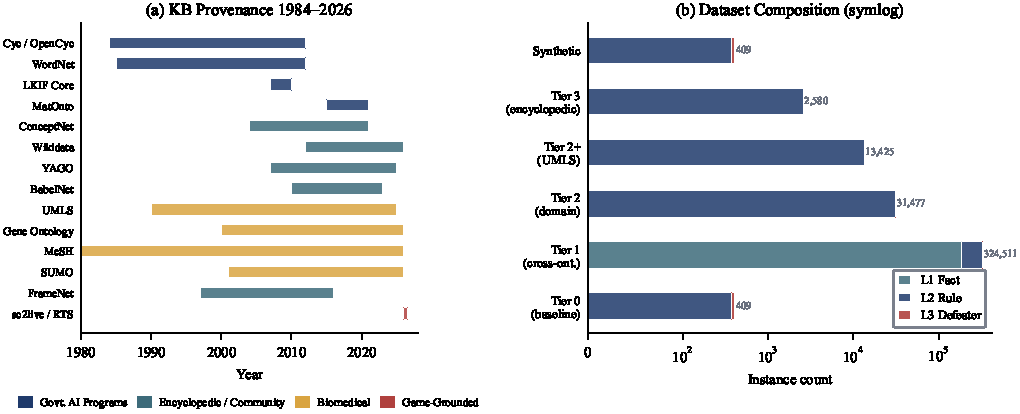
\includegraphics[width=\textwidth]{figures/fig_sources.pdf}
\caption{(a)~Provenance timeline of 18 knowledge base sources spanning 1984 (Cyc) to 2025 (UMLS 2025AB), color-coded by source class: government AI programs (blue), encyclopedic / community (teal), biomedical (gold), and game-grounded (red). (b)~Dataset composition by tier and instance level on a symlog scale. Tier~1 (cross-ontology) provides the majority of instances; Level~3 (defeater abduction) appears only in Tier~0 and the matched synthetic control.}
\label{fig:sources}
\end{figure}

DeFAb is built on the deliberate inheritance of four decades of publicly funded knowledge engineering. The provenance timeline in Figure~\ref{fig:sources}(a) traces this lineage through the four programmatic threads identified in Section~\ref{sec:intro}: government AI initiatives of the 1980s and 1990s (Cyc, WordNet, LKIF Core, MatOnto), encyclopedic and community projects (ConceptNet, Wikidata, YAGO, BabelNet, FrameNet, SUMO), biomedical infrastructure (UMLS, Gene Ontology, MeSH), and the recent game-grounded family that complements them with vocabulary-disjoint contemporary content. Our objective is not to enumerate these resources but to convert each into a uniformly structured defeasible-theory representation that the same pipeline, the same verifier, and the same curriculum can consume. The four extraction tiers below reflect the priority and scale of this conversion rather than any qualitative distinction between sources.

The baseline tier comprises expert-curated instances drawn from YAGO~4.5, WordNet~3.0, LKIF Core, and MatOnto. It contributes 2{,}318 rules and the 409 evaluation instances (374 Level~2, 35 Level~3) used for our primary evaluation, frozen at v1.0 for cross-study comparability.

Tier~1, the primary scale mechanism, pairs the OpenCyc hierarchy~\cite{lenat1995cyc} (239K terms) with ConceptNet~5.8~\cite{speer2017conceptnet} (34M edges), traversing ancestor chains to inherit behavioral properties. The procedure yields strict taxonomic rules from \texttt{IsA} edges, defeasible behavioral rules from \texttt{CapableOf} and \texttt{HasProperty} edges, and defeaters from \texttt{NotCapableOf} edges, across five domains: biology, legal reasoning, materials science, chemistry, and everyday commonsense. Tier~2 adds domain-specific rules and structured defeaters from the Gene Ontology~\cite{ashburner2000go} (using \texttt{NOT}-qualified annotations), MeSH, SUMO~\cite{niles2001sumo}, FrameNet~\cite{baker1998framenet}, Wikidata~\cite{vrandecic2014wikidata} (whose P2303 ``exception to constraint'' property is the highest-quality automatic defeater source we have identified), UMLS~\cite{lindberg1993umls} (189 biomedical vocabularies, 29.5M rules), and BabelNet~\cite{navigli2012babelnet}. Tier~3 contributes 3.5M rules from full YAGO~4.5 extraction.

A separate game-grounded family (Tier RTS) shares the defeasible-theory schema with the naturalistic tiers but at zero predicate vocabulary overlap with them. The hand-authored \texttt{rts\_engagement} Rules-of-Engagement KB (148 rules, 162 facts, 6 hand-crafted Level~3 seed conflicts) is formally certified by \texttt{scripts/certify\_rts\_kb.py}; the Lux~AI Season~3 (NeurIPS~2024) competition rules add roughly 130 further rules; and a live StarCraft~II bridge (\texttt{src/blanc/sc2live/}) lifts game state into ground facts via an \texttt{ObservationLifter} and ingests replays via a \texttt{ReplayTraceExtractor}, generating several thousand Level~1 and Level~2 instances per game session. The vocabulary disjointness of this family makes it a useful instrument for testing whether reported accuracy on the naturalistic tiers reflects defeasible reasoning or surface vocabulary recognition.

\begin{table}[t]
\centering
\small
\caption{Knowledge base pipeline: extraction results by tier. The RTS row aggregates three game-grounded KBs; \texttt{sc2live} counts are session-dependent ($^{\ddagger}$). UMLS requires NLM license (obtained). $^{\dagger\dagger}$RTS rule total counts \texttt{rts\_engagement}+\texttt{lux\_ai\_s3} only.}
\label{tab:kbsummary}
\begin{tabular}{@{}llrr@{}}
\toprule
Tier & Primary Sources & Rules & Instances \\
\midrule
0 (baseline) & YAGO, WordNet, LKIF, MatOnto & 2,318 & 409 \\
1 (cross-ontology) & OpenCyc + ConceptNet & 289,305 & 324,511 \\
2 (domain-specific) & GO, MeSH, SUMO, FrameNet, Wikidata, BabelNet & 535,565 & 31,477 \\
2+ (biomedical) & UMLS 2025AB & 29,465,582 & 13,425 \\
3 (encyclopedic) & YAGO 4.5 full & 3,457,940 & 2,580 \\
RTS (game) & rts\_engagement, lux\_ai\_s3, sc2live$^{\ddagger}$ & 478$^{\dagger\dagger}$ & 246+$^{\ddagger}$ \\
\midrule
\multicolumn{2}{@{}l}{Materialized total (Tiers 0--3 + RTS)} & 33,751,188 & 372,648+$^{\ddagger}$ \\
\bottomrule
\end{tabular}
\end{table}

Across all tiers, the richest automated defeater sources are Wikidata P2303 constraint--exception pairs (11{,}557 defeaters), Gene Ontology \texttt{NOT}-qualified annotations (1{,}250), and SUMO axioms (792). Combined with ConceptNet \texttt{NotCapableOf} (approximately 300{,}000 edges), these constitute, to our knowledge, the largest publicly available collection of structured defeasible exceptions assembled for benchmark generation.


%% ====================================================================
\section{Worked Example: IDP Defeater Abduction}\label{sec:example}
%% ====================================================================

\begin{figure}[t]
\centering
\resizebox{\textwidth}{!}{% Figure 4: IDP defeater abduction worked example.
% Appendix-sized figure (text-width). 2x2 panel grid with absolute coords.
% No nested tikzpictures. Score boxes are inline \colorbox labels.
%
% Grid (anchor=north west on every panel):
%   Top-left  (i)   Complete theory D_full     at (0,    0)
%   Top-right (ii)  Challenge theory D-        at (8.0,  0)
%   Bot-left  (iii) Anomaly surfaces           at (0,   -5.5)
%   Bot-right (iv)  Graded resolutions         at (8.0, -5.5)
%
% Each panel: 7.0cm wide, 5.0cm tall, anchored top-left.
% Inter-panel horizontal gap: 1.0cm (8.0 - 7.0). Vertical gap: 0.5cm.
% Arrows are drawn last, between named anchors.
%
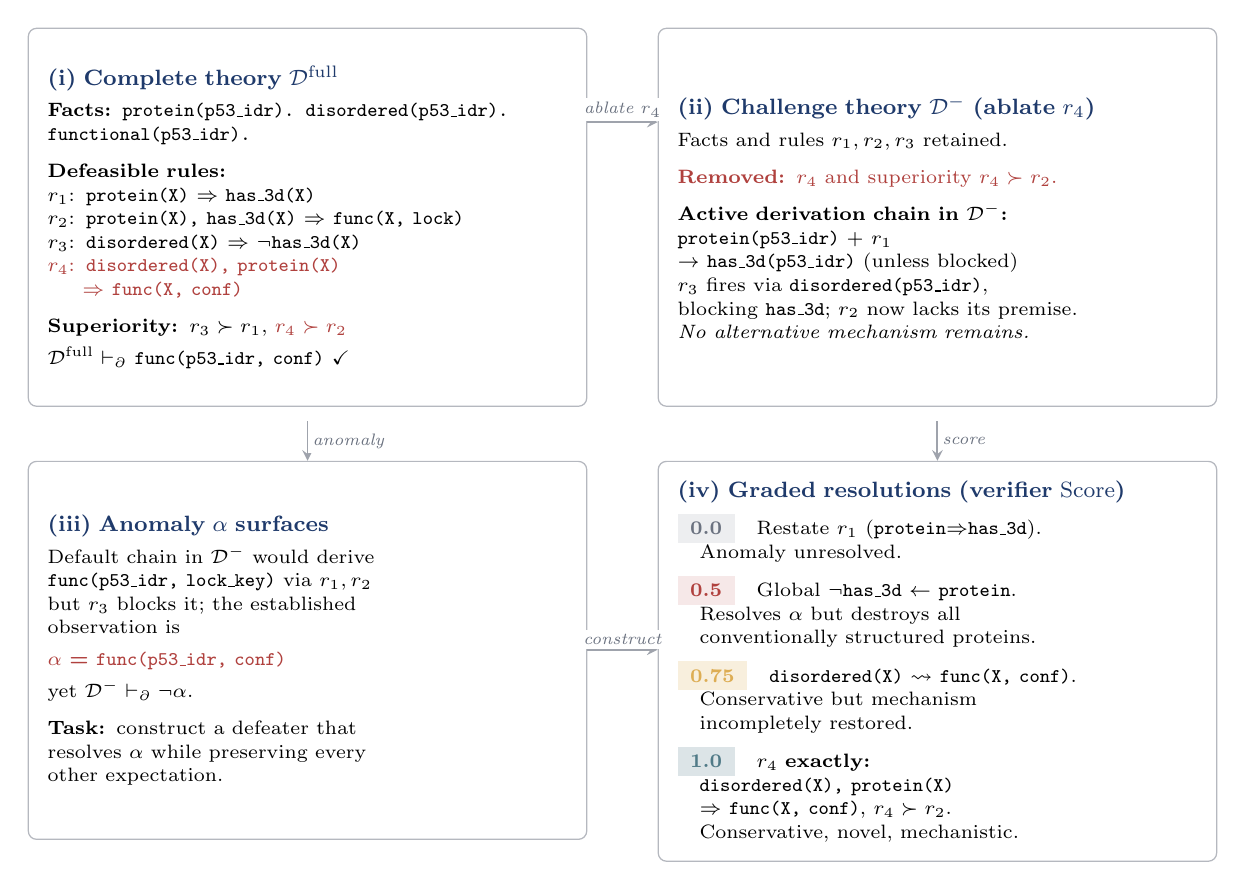
\begin{tikzpicture}[
    >=stealth,
    panel/.style={
        draw=defabGray!50, rounded corners=3pt,
        inner sep=7pt, align=left, fill=white,
        font=\fontsize{7}{8.5}\selectfont,
        line width=0.45pt,
        text width=6.6cm, minimum height=4.8cm, anchor=north west
    },
    % inter-panel arrows
    flow/.style={->, thick, color=defabGray!65, line width=0.7pt},
    flowlbl/.style={
        font=\fontsize{6.5}{7.5}\selectfont\itshape,
        text=defabGray, fill=white, inner sep=1.5pt
    },
]

%% =================================================================
%% Panel (i): Complete theory D_full   (top-left)
%% =================================================================
\node[panel] at (0, 0) (p1) {
  {\fontsize{8}{9.5}\selectfont\bfseries\color{defabBlue}(i) Complete theory $\Dfull$}\\[3pt]
  \textbf{Facts:} \texttt{protein(p53\_idr).} \texttt{disordered(p53\_idr).}\\
  \texttt{functional(p53\_idr).}\\[5pt]
  \textbf{Defeasible rules:}\\
  $r_1$: \texttt{protein(X) $\Rightarrow$ has\_3d(X)}\\
  $r_2$: \texttt{protein(X), has\_3d(X) $\Rightarrow$ func(X, lock)}\\
  $r_3$: \texttt{disordered(X) $\Rightarrow$ $\neg$has\_3d(X)}\\
  {\color{defabRed}$r_4$: \texttt{disordered(X), protein(X)}}\\
  \phantom{$r_4$:\ }{\color{defabRed}\texttt{$\Rightarrow$ func(X, conf)}}\\[5pt]
  \textbf{Superiority:} $r_3 \succ r_1$, {\color{defabRed}$r_4 \succ r_2$}\\[3pt]
  $\Dfull \pPartial$ \texttt{func(p53\_idr, conf)} \checkmark
};

%% =================================================================
%% Panel (ii): Challenge theory D-   (top-right)
%% =================================================================
\node[panel] at (8.0cm, 0) (p2) {
  {\fontsize{8}{9.5}\selectfont\bfseries\color{defabBlue}(ii) Challenge theory $\Dm$ (ablate $r_4$)}\\[3pt]
  Facts and rules $r_1, r_2, r_3$ retained.\\[5pt]
  {\color{defabRed}\textbf{Removed:} $r_4$ and superiority $r_4 \succ r_2$.}\\[5pt]
  \textbf{Active derivation chain in $\Dm$:}\\
  \texttt{protein(p53\_idr)} + $r_1$\\
  $\to$ \texttt{has\_3d(p53\_idr)} (unless blocked)\\
  $r_3$ fires via \texttt{disordered(p53\_idr)},\\
  blocking \texttt{has\_3d}; $r_2$ now lacks its premise.\\
  \emph{No alternative mechanism remains.}
};

%% =================================================================
%% Panel (iii): Anomaly surfaces   (bottom-left)
%% =================================================================
\node[panel] at (0, -5.5cm) (p3) {
  {\fontsize{8}{9.5}\selectfont\bfseries\color{defabBlue}(iii) Anomaly $\alpha$ surfaces}\\[3pt]
  Default chain in $\Dm$ would derive\\
  \texttt{func(p53\_idr, lock\_key)} via $r_1, r_2$\\
  but $r_3$ blocks it; the established\\
  observation is\\[3pt]
  {\color{defabRed}\textbf{$\alpha$ = \texttt{func(p53\_idr, conf)}}}\\[3pt]
  yet $\Dm \pPartial \neg\alpha$.\\[5pt]
  \textbf{Task:} construct a defeater that\\
  resolves $\alpha$ while preserving every\\
  other expectation.
};

%% =================================================================
%% Panel (iv): Graded resolutions   (bottom-right)
%% =================================================================
\node[panel] at (8.0cm, -5.5cm) (p4) {
  {\fontsize{8}{9.5}\selectfont\bfseries\color{defabBlue}(iv) Graded resolutions (verifier $\Score$)}\\[3pt]
  \colorbox{defabGray!12}{\textcolor{defabGray}{\bfseries\,0.0\,}}\quad
  Restate $r_1$ (\texttt{protein$\Rightarrow$has\_3d}).\\
  \quad Anomaly unresolved.\\[4pt]
  \colorbox{defabRed!12}{\textcolor{defabRed}{\bfseries\,0.5\,}}\quad
  Global \texttt{$\neg$has\_3d $\leftarrow$ protein}.\\
  \quad Resolves $\alpha$ but destroys all\\
  \quad conventionally structured proteins.\\[4pt]
  \colorbox{defabGold!18}{\textcolor{defabGold!90}{\bfseries\,0.75\,}}\quad
  \texttt{disordered(X) $\leadsto$ func(X, conf)}.\\
  \quad Conservative but mechanism\\
  \quad incompletely restored.\\[4pt]
  \colorbox{defabTeal!18}{\textcolor{defabTeal!90}{\bfseries\,1.0\,}}\quad
  \textbf{$r_4$ exactly:}\\
  \quad \texttt{disordered(X), protein(X)}\\
  \quad \texttt{$\Rightarrow$ func(X, conf)}, $r_4 \succ r_2$.\\
  \quad Conservative, novel, mechanistic.
};

%% =================================================================
%% Inter-panel arrows  (drawn last, between named anchors)
%% =================================================================
% (i) -> (ii) horizontal arrow at top
\draw[flow] (p1.east |- 0,-1.2) -- node[flowlbl, above] {ablate $r_4$}
            (p2.west |- 0,-1.2);

% (i) -> (iii) vertical arrow at left
\draw[flow] (p1.south |- 0,-5.0) -- node[flowlbl, right] {anomaly}
            (p3.north |- 0,-5.5);

% (ii) -> (iv) vertical arrow at right
\draw[flow] (p2.south |- 0,-5.0) -- node[flowlbl, right] {score}
            (p4.north |- 0,-5.5);

% (iii) -> (iv) horizontal arrow at bottom
\draw[flow] (p3.east |- 0,-7.9) -- node[flowlbl, above] {construct}
            (p4.west |- 0,-7.9);

\end{tikzpicture}
}
\caption{Level~3 defeater abduction: the intrinsically disordered protein (IDP) discovery as a four-stage walkthrough. (i)~Complete theory $\Dfull$ with defeasible rules and the IDP defeater $r_4$; (ii)~Ablation: $r_4$ and its superiority are removed, forming challenge theory $\Dm$; (iii)~Anomaly surfaces: $\Dm$ predicts lock-key mechanism for p53\_idr despite \texttt{disordered(p53\_idr)}, which is anomalous; (iv)~Graded resolutions scored by the polynomial-time verifier. Score 0: restates the default (anomaly unresolved). Score 0.5: overly broad defeater destroys other predictions. Score 0.75: valid weak conservative resolution, but misses the causal mechanism. Score 1.0: the IDP defeater --- conservative, novel, mechanistically precise.}
\label{fig:level3example}
\end{figure}

We use the IDP discovery, first introduced in Section~\ref{sec:intro}, as a running example to illustrate the four stages of a Level~3 task and the operation of the graded scoring function (Figure~\ref{fig:level3example}).

Consider the biochemistry program $\Pi_{\mathrm{bio}}$ with facts \texttt{protein(p53\_idr)}, \texttt{disordered(p53\_idr)}, and \texttt{functional(p53\_idr)}, together with the rules
\begin{align*}
    r_1&: \texttt{prot}(X) \defto \texttt{has\_3d}(X), \quad
    r_2: \texttt{prot}(X), \texttt{has\_3d}(X) \defto \texttt{func}(X, \texttt{lock}) \\
    r_3&: \texttt{disordered}(X) \defto \neg\texttt{has\_3d}(X), \quad
    r_4: \texttt{disordered}(X), \texttt{prot}(X) \defto \texttt{func}(X, \texttt{conf})
\end{align*}
and the superiority assertions $r_3 \succ r_1$ and $r_4 \succ r_2$. Under the complete theory $\Dfull$, \texttt{p53\_idr} is correctly derived to function via the conformational-ensemble mechanism. To form a Level~3 instance we remove $r_4$ together with its superiority assertion, leaving the challenge theory $\Dm$. In $\Dm$ the chain through $r_1$ and $r_2$ would derive a lock-and-key mechanism for p53\_idr were it not for $r_3$, which blocks the stable-3D-structure conclusion; the result is that no functional mechanism can be derived for p53\_idr at all. The observation $\alpha = \texttt{func}(\texttt{p53\_idr}, \texttt{conf})$ is therefore anomalous in $\Dm$, and the model is asked to construct a defeater that resolves the anomaly while preserving the rest of the theory's expectations.

The graded scoring function rewards surgical precision rather than mere anomaly resolution. A response that simply restates the default rule $r_1$ scores~0 because the anomaly remains unresolved. A global defeater of the form $\neg\texttt{has\_3d}(X) \leftarrow \texttt{protein}(X)$ resolves the anomaly but destroys predictions for all conventionally structured proteins, scoring~0.5 on the conservativity criterion. A narrower defeater $\texttt{disordered}(X) \defeatto \texttt{func}(X, \texttt{conf})$ is conservative but only partially restores the expected conclusion about p53\_idr's mechanism, earning a weak-conservative score of~0.75. Only the full rule $r_4$ with its superiority $r_4 \succ r_2$ scores~1.0: it is conservative, novel in the sense that $\Nov > 0$ if \texttt{conf} is a new predicate, and mechanistically precise. The full graded rubric appears in panel~(iv) of Figure~\ref{fig:level3example}, and a parallel three-level walkthrough on a simpler bear-hibernation theory is given in Appendix~\ref{app:example}.


%% ====================================================================
\section{Baseline Evaluation}\label{sec:evaluation}
%% ====================================================================

Before presenting model-by-model results we establish the structural context. The symbolic baseline --- an Answer Set Programming solver (clingo) implementing the same defeasible derivation algorithm we use to generate the instances --- achieves 100\% accuracy on all 374 Level~2 and all 35 Level~3 instances in under 50 microseconds per instance~\cite{maher2001propositional}. The instances are not difficult by the standards of formal reasoning; they are difficult for language models because language models do not perform formal reasoning. Every gap reported below is a gap to a microsecond rule-based solver, not to a more capable model.

%% --------------------------------------------------------------------
\subsection{Experimental Setup}\label{subsec:setup}
%% --------------------------------------------------------------------

We evaluate four frontier models. The reasoning-optimized GPT-5.2-chat~\cite{openai2025gpt52} and Kimi-K2.5~\cite{moonshot2025kimi} are closed-source and accessed via Azure AI Foundry, as is the instruction-optimized Claude~Sonnet~4.6~\cite{anthropic2024claude}; the reasoning-optimized DeepSeek-R1-Distill-Llama-70B~\cite{deepseek2025r1} is open-source and served via vLLM on CURC Alpine (NVIDIA A100 80\,GB). All models use greedy decoding with temperature zero. Each instance is presented under all four text rendering modalities (M1--M4) and under two prompting strategies, direct and chain-of-thought. The chain-of-thought scaffold mirrors the structure of defeasible derivation itself: identify applicable rules, determine missing or blocking elements, check attackers and superiority, and propose a conservative hypothesis.

%% --------------------------------------------------------------------
\subsection{Primary Results}\label{subsec:results}
%% --------------------------------------------------------------------

\begin{figure}[t]
\centering
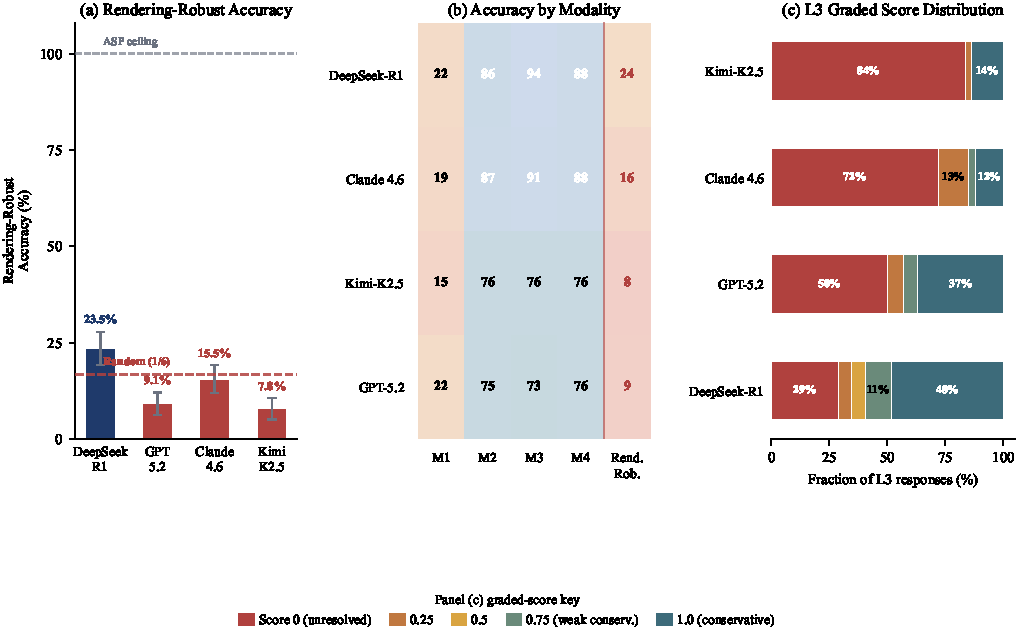
\includegraphics[width=\textwidth]{figures/fig_results.pdf}
\caption{(a)~Level~3 accuracy by prompting strategy. Dashed lines mark 16.7\% (random 1/6 baseline) and 100\% (ASP symbolic ceiling). Reasoning-optimized models gain +56 to +79~pp under CoT; the instruction-optimized Claude \emph{regresses} by $-14$~pp. (b)~Accuracy by rendering modality M1--M4, with the rendering-robust worst-case added as a rightmost column. All models collapse to 14--22\% on M1 (near-random) versus 73--94\% on M2--M4. (c)~Graded-score distribution at Level~3 per model. The ``Score~0'' (anomaly unresolved) fraction dominates for Claude (84.4\%) and Kimi (85.9\%).}
\label{fig:results}
\end{figure}

\begin{table}[t]
\centering
\caption{Accuracy (\%) by model and task level. \emph{Rend.-Rob.} = rendering-robust (worst case over M1--M4); random chance = 16.7\%; ASP symbolic ceiling = 100\%. Wilson 95\% CI half-widths: $\pm 4$~pp at Level~2; $\pm 15$--$17$~pp at Level~3. All Level~3 pairwise differences significant by McNemar's test ($p < 0.001$) except Claude vs.\ Kimi ($p = 0.556$).}
\label{tab:main}
\begin{tabular}{lcccccc}
\toprule
Model & L2 Direct & L2 CoT & L3 Direct & L3 CoT & L3 Best & Rend.-Rob. \\
\midrule
ASP Symbolic Ceiling & 100\% & --- & 100\% & --- & 100\% & 100\% \\
\midrule
DeepSeek-R1         & 73.7\% & 71.4\% & 37.1\% & \textbf{92.9\%} & \textbf{65.0\%} & 23.5\% \\
GPT-5.2-chat        & \textbf{78.5\%} & 47.5\% & \phantom{0}7.9\% & 87.1\% & 47.5\% & \phantom{0}9.1\% \\
Claude~Sonnet~4.6   & 79.3\% & 52.3\% & \textbf{23.6\%} & \phantom{0}9.3\% & 16.4\% & 15.5\% \\
Kimi-K2.5           & 71.9\% & 70.4\% & \phantom{0}0.8\% & 27.6\% & 14.2\% & \phantom{0}7.8\% \\
\midrule
Random (1/6) & \multicolumn{5}{c}{16.7\%} & 16.7\% \\
\bottomrule
\end{tabular}
\end{table}

%% --------------------------------------------------------------------
\subsection{Key Findings}\label{subsec:findings}
%% --------------------------------------------------------------------

The single most important number in our evaluation is the rendering-robust accuracy, computed as the worst-case accuracy over the four text modalities M1--M4. It is 7.8\% for Kimi, 9.1\% for GPT-5.2, 15.5\% for Claude, and 23.5\% for DeepSeek-R1. Two of four models are at or below the 16.7\% random-chance baseline for six-choice selection, and the best of the four exceeds it only modestly. The much higher accuracy figures reported for individual formal modalities (73--94\% at Level~2 in M2--M4) therefore do not reflect defeasible reasoning capability so much as the exploitation of surface syntax patterns: when the same logical content is presented as English prose in M1, performance collapses to near-random levels. Whatever the formal-modality scores measure, it is not robust to surface form.

This pattern is reinforced by the Level~3 results under direct prompting. Kimi achieves 0.8\% on Level~3 direct (one correct response out of 125 attempts), GPT-5.2 achieves 7.9\%, and even DeepSeek-R1 manages only 37.1\%. Direct-prompting belief revision is essentially absent for three of the four models. The error taxonomy in Table~\ref{tab:level3_metrics} explains why the absence is so deep: 80.9\% of Kimi's Level~3 responses fall into class E1 (decoder failure), meaning the model cannot produce outputs that can be parsed as valid hypotheses at all. This is a metacognitive failure distinct from incorrect reasoning --- the model does not recognize what output format is being requested.

Chain-of-thought prompting reveals an architectural dissociation rather than a uniform improvement. CoT raises Level~3 accuracy by 56~pp for DeepSeek-R1 and 79~pp for GPT-5.2, both reasoning-optimized models, while \emph{lowering} Claude's accuracy by 14~pp. The same prompting scaffold that enables belief revision in one architecture destroys it in another. This effect is too large to attribute to task difficulty; it is an architectural fingerprint of how each model integrates explicit reasoning steps with selection-style outputs.

The narrative modality is a universal bottleneck. All models score between 14\% and 22\% on M1 (Figure~\ref{fig:results}b), a 55--70~pp drop from their performance on the formal modalities. This is the largest single effect in the evaluation, exceeding any inter-model or inter-level difference. The error breakdown is informative: M1 generates 11{,}765 decoder failures versus 4{,}779 for M4 on the same instances, suggesting that models cannot reliably extract their own intended meaning from English-prose presentations of the same logical theory. The collapse is consistent with surface pattern matching against Prolog syntax being the operative mechanism on M2--M4.

A second universal CoT effect appears at Level~2: chain-of-thought prompting decreases Level~2 accuracy by between 1.5 and 31 percentage points for every model. For structured selection tasks where surface string alignment between output and candidate suffices, verbal elaboration disrupts that alignment. This replicates the overthinking effect~\cite{chen2024overthinking} and confirms that the benefits of chain-of-thought prompting are highly task-type-specific.

The one apparent area of strength is Level~2 grounding under direct prompting on formal modalities, where all four models achieve 71.9--79.3\% accuracy. We report this finding last and with explicit qualification: the same number falls to between 7.8\% and 23.5\% under the rendering-robust metric, and the symbolic solver achieves 100\% with no training whatsoever. The graded scoring distribution at Level~3 (Figure~\ref{fig:results}c) is particularly stark in this regard. The fraction of responses scoring exactly zero (anomaly entirely unresolved) is 84\% for Claude and 86\% for Kimi. These models are not producing near-miss conservative resolutions; they are failing the task entirely. Table~\ref{tab:level3_metrics} reports the full Level~3 metric suite.

\begin{table}[t]
\centering
\caption{Level~3 formal metrics by model. \emph{Res}: anomaly resolved; \emph{Cons}: conservative; $\overline{\Nov}$: mean novelty; \emph{E1/E2/E5}: error class breakdown (\%).}
\label{tab:level3_metrics}
\begin{tabular}{lrrrrrrrrr}
\toprule
Model & Acc & Res & Cons & $\overline{\Nov}$ & E1 & E2 & E5 \\
\midrule
DeepSeek-R1 & 65.0\% & 59.6\% & 59.6\% & 0.14 & 16.8\% & 23.6\% & 11.4\% \\
GPT-5.2-chat & 47.5\% & 42.9\% & 42.9\% & 0.23 & 26.1\% & 31.1\% & \phantom{0}6.1\% \\
Claude~Sonnet~4.6 & 16.4\% & 15.0\% & 15.0\% & 0.44 & 26.8\% & 58.2\% & \phantom{0}2.9\% \\
Kimi-K2.5 & 14.2\% & 13.9\% & 13.9\% & 0.11 & 80.9\% & \phantom{0}5.2\% & \phantom{0}0.0\% \\
\bottomrule
\end{tabular}
\end{table}

The synthetic contamination control methodology is established but its empirical evaluation is still in progress: we have generated 409 structurally matched synthetic instances with invented predicate names (Section~\ref{subsec:synthetic}), and methodology validation confirms that the synthetic theories preserve the structural difficulty distributions of their naturalistic counterparts while using entirely novel vocabulary. Frontier-model evaluation on these synthetic instances and computation of the per-model contamination gap $\Delta_{\mathrm{synth}}$ are scheduled for the next revision.


%% ====================================================================
\section{DeFAb as a Finetuning Substrate}\label{sec:finetuning}
%% ====================================================================

\begin{figure}[t]
\centering
\resizebox{\textwidth}{!}{% Figure 7: Verifier-as-reward diagram for the finetuning substrate.
% Absolute coordinates throughout; explicit \draw arrows between named anchors.
%
% Layout (vertical positions chosen so strips never overlap output boxes):
%   Properties strip   at (0,    3.0)   width 10cm height 0.55cm  (clears box i top y=2.425)
%   Input box          at (-5.5, 0)     width 3.0cm height 1.2cm
%   Central verifier   at (0,    0)     width 4.2cm height 1.4cm
%   Four output boxes  at (5.7, +1.95 / +0.65 / -0.65 / -1.95)  width 4.6cm height 0.95cm
%   Curriculum strip   at (0,   -3.0)   width 10cm height 0.55cm (clears box iv bottom y=-2.425)
%
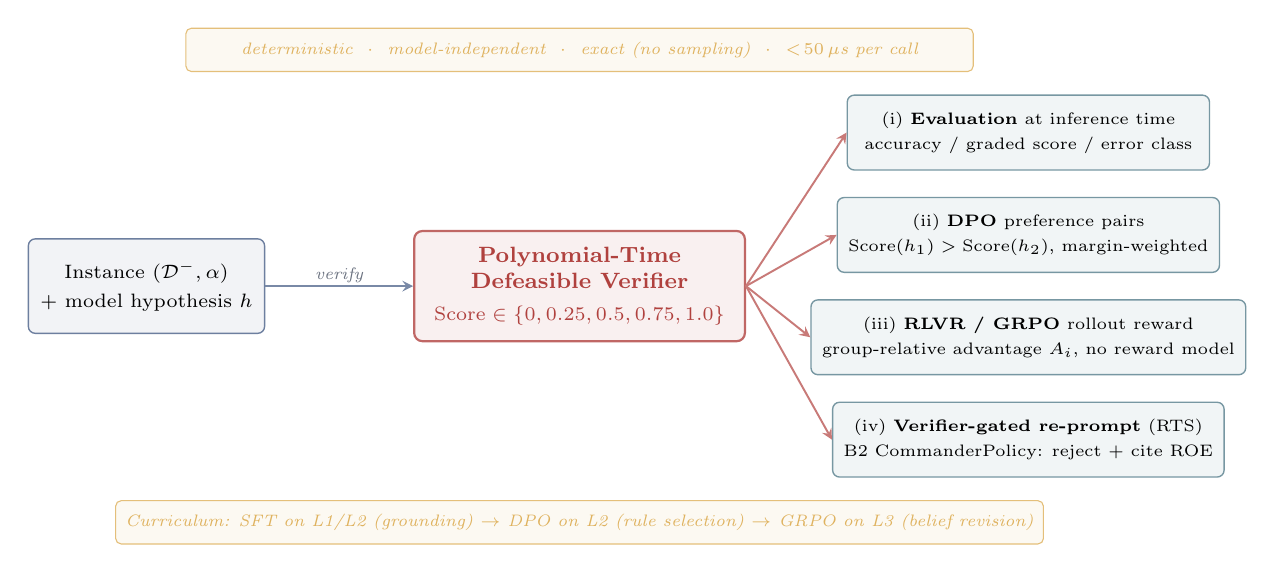
\begin{tikzpicture}[
    >=stealth,
    verifier/.style={
        draw=defabRed!80, rounded corners=3pt,
        font=\fontsize{8}{9.5}\selectfont\bfseries,
        inner sep=5pt, fill=defabRed!8, line width=0.8pt,
        text=defabRed, text centered, align=center
    },
    inputbox/.style={
        draw=defabBlue!65, rounded corners=2.5pt,
        font=\fontsize{7}{8.5}\selectfont,
        inner sep=4pt, fill=defabBlue!6, line width=0.5pt,
        text centered, align=center
    },
    outputbox/.style={
        draw=defabTeal!70, rounded corners=2.5pt,
        font=\fontsize{6.5}{8}\selectfont,
        inner sep=4pt, fill=defabTeal!7, line width=0.5pt,
        text centered, align=center
    },
    propbox/.style={
        draw=defabGold!70, rounded corners=2pt,
        font=\fontsize{6.5}{7.5}\selectfont\itshape,
        inner sep=3.5pt, fill=defabGold!7, line width=0.4pt,
        text=defabGold!85, text centered, align=center
    },
    arr/.style={->, thick, color=defabRed!70, line width=0.7pt},
    arrin/.style={->, thick, color=defabBlue!60, line width=0.7pt},
    arrlbl/.style={
        font=\fontsize{6}{7}\selectfont\itshape,
        text=defabGray, fill=white, inner sep=1pt
    },
]

%% =================================================================
%% Properties strip (top)
%% =================================================================
\node[propbox, minimum width=10cm, minimum height=0.55cm] (props)
    at (0, 3.0)
    {deterministic\ \ $\cdot$\ \ model-independent\ \ $\cdot$\ \ exact (no sampling)\ \ $\cdot$\ \ $<\!50\,\mu$s per call};

%% =================================================================
%% Input box (left)
%% =================================================================
\node[inputbox, minimum width=3.0cm, minimum height=1.2cm] (inst)
    at (-5.5, 0)
    {Instance $(\Dm, \alpha)$\\[2pt] + model hypothesis $h$};

%% =================================================================
%% Central verifier
%% =================================================================
\node[verifier, minimum width=4.2cm, minimum height=1.4cm] (ver)
    at (0, 0)
    {Polynomial-Time\\Defeasible Verifier\\[2pt]
     {\fontsize{7}{8}\selectfont $\Score \in \{0, 0.25, 0.5, 0.75, 1.0\}$}};

%% Input -> verifier
\draw[arrin] (inst.east) -- node[arrlbl, above] {verify} (ver.west);

%% =================================================================
%% Four output boxes (right column, stacked vertically)
%% =================================================================
\node[outputbox, minimum width=4.6cm, minimum height=0.95cm] (eval)
    at (5.7, 1.95)
    {(i) \textbf{Evaluation} at inference time\\[1pt]
     accuracy / graded score / error class};

\node[outputbox, minimum width=4.6cm, minimum height=0.95cm] (dpo)
    at (5.7, 0.65)
    {(ii) \textbf{DPO} preference pairs\\[1pt]
     $\Score(h_1) > \Score(h_2)$, margin-weighted};

\node[outputbox, minimum width=4.6cm, minimum height=0.95cm] (grpo)
    at (5.7, -0.65)
    {(iii) \textbf{RLVR / GRPO} rollout reward\\[1pt]
     group-relative advantage $A_i$, no reward model};

\node[outputbox, minimum width=4.6cm, minimum height=0.95cm] (gate)
    at (5.7, -1.95)
    {(iv) \textbf{Verifier-gated re-prompt} (RTS)\\[1pt]
     B2 CommanderPolicy: reject + cite ROE};

%% Verifier -> each output (explicit anchors)
\draw[arr] (ver.east) -- (eval.west);
\draw[arr] (ver.east) -- (dpo.west);
\draw[arr] (ver.east) -- (grpo.west);
\draw[arr] (ver.east) -- (gate.west);

%% =================================================================
%% Curriculum strip (bottom)
%% =================================================================
\node[propbox, minimum width=10cm, minimum height=0.55cm] (curr)
    at (0, -3.0)
    {Curriculum: SFT on L1/L2 (grounding) $\to$ DPO on L2 (rule selection) $\to$ GRPO on L3 (belief revision)};

\end{tikzpicture}
}
\caption{The polynomial-time verifier as an exact reward function for all preference optimization paradigms. The same Stage~3 verifier (no approximation, no sampling, deterministic) feeds: (i)~evaluation scoring at inference time; (ii)~margin-weighted DPO preference pairs from the graded $\Score$ function; (iii)~RLVR/GRPO rollout rewards, eliminating reward model approximation error; (iv)~verifier-gated re-prompt feedback for LLM-as-commander policies in the RTS game-grounded track. DeFAb is the finetuning substrate the RLVR paradigm needs.}
\label{fig:finetuning}
\end{figure}

The failure cascade documented in Section~\ref{sec:evaluation} establishes the need for training, not merely better evaluation. DeFAb provides the substrate. The same polynomial-time verifier that scores every evaluation instance also serves as an exact reward function, eliminating the reward-model approximation error that undermines recent RLVR systems~\cite{ouyang2022training, zheng2025verifybench, rlbff2025}.

Direct preference optimization is the most immediate application. Given two responses $h_1, h_2$ to the same Level~3 instance, the verifier produces ordered scores $\Score(h_1) \geq \Score(h_2)$, so responses with $\Score(h) = 1.0$ become preferred completions and responses with $\Score(h) = 0$ become rejected ones. The graded scale enables a margin-weighted variant of DPO in which the preference margin $m = \Score(h_1) - \Score(h_2)$ weights the loss, rewarding larger score separations more strongly than near-ties. This is a strict strengthening of binary DPO for tasks that admit a measurable quality gradient.

The same verifier serves directly as the GRPO reward function~\cite{shao2024deepseekmath}. For a rollout group of $G$ candidate defeaters generated for the same instance, the group-relative advantage $A_i = \Score(h_i) - \frac{1}{G}\sum_j \Score(h_j)$ is computable in microseconds, with no reward model, no judge LLM, and no temperature sampling from a separate model. The contrast with verifier-LLM approaches such as the AIME CoT Verification dataset~\cite{wen2025aimecot}, in which separate verifier LLMs disagree on 15--20\% of instances, is qualitative rather than quantitative: DeFAb's verifier is deterministic, so the same input always produces the same score, and any disagreement vanishes by construction.

The three-level hierarchy supplies a natural curriculum. Supervised finetuning on Level~1 and Level~2 instances establishes grounding, DPO on Level~2 contrastive pairs refines rule selection, and GRPO on Level~3 instances trains belief revision under the exact reward. Within each level, theory size and support depth can be controlled parametrically to stage difficulty. Beyond curriculum learning, the structure of defeasible reasoning admits a second self-play mechanism: defeasible conflicts --- theory states in which both $q$ and $\comp{q}$ are derivable --- constitute two-player zero-sum games whose outcomes generate structurally grounded preference pairs without requiring a separate curriculum designer.

Finally, the verifier extends naturally to real-time deployment. The \texttt{CommanderPolicy} in \texttt{src/blanc/sc2live/policies/commander.py} implements three enforcement modes for LLM-as-commander policies in the StarCraft~II RTS track: a trust-LLM mode (B0) that applies orders verbatim and logs compliance only post-hoc, an audit-only mode (B1) that scores each order against the verifier without acting on the score, and a verifier-gated mode (B2) that rejects non-compliant orders and re-prompts the model up to three times with the specific ROE violation reason. We pre-register the hypotheses that B2 compliance exceeds B1 and B0 compliance, and that the mean number of re-prompts per game tick decreases over the course of a game as the model adapts in context. This extends the verifier-as-reward principle to closed-loop game-grounded deployment, with the same verifier feeding evaluation, preference data, RL rewards, and runtime gating.

Taken together, DeFAb supplies what current RLVR systems lack for defeasible reasoning: a domain-spanning, contamination-resistant, formally verified reward signal with polynomial-time computation, graded quality measurement, a natural curriculum, and over 372{,}000 instances spanning five naturalistic domains and a vocabulary-disjoint game-grounded track to mitigate the risk of domain overfitting during training.


%% ====================================================================
\section{Discussion}\label{sec:discussion}
%% ====================================================================

The results we have reported should be read as an upper bound on current frontier model capability. The 35-instance Level~3 evaluation uses instances with mean predicate novelty $\Nov^* = 0.14$ (range $[0, 0.5]$), mean support size 6.7 (maximum 10), and a single anomaly per instance. By construction, this distribution rewards the Lakatosian monster-barring strategy --- restricting the original rule's domain using existing predicates --- which is the simplest possible form of belief revision. The 92.9\% Level~3 CoT figure for DeepSeek-R1 is therefore better understood as an artifact of an easy difficulty distribution than as evidence of robust belief revision capability. Properly bounding the structural gap requires evaluating models on instances that demand lemma-incorporation rather than monster-barring.

To this end we pre-register \textsc{DeFAb-Hard}, a structurally hardened Level~3 subset stratified along four orthogonal hardening axes. The first axis (H1) imposes a high-novelty requirement, $\Nov(r^*, \Dm) \geq 0.5$ with novel predicate vocabulary verified against Common Crawl, targeting 1{,}000 instances spread across five domains. The second axis (H2) scales theory size and support depth to $|\D| \in \{50, 100, 200\}$ with depth at least five and at least three competing defaults, targeting 100 instances per scale tier. The third axis (H3) introduces multi-anomaly instances with $k \geq 3$ unrelated anomalies, ensuring that conservativity is no longer a default pass; the target is 100 instances. The fourth axis (H4) completes the contamination evaluation by running the four-model panel on the 409 structurally matched synthetic instances we have already generated, in order to compute the per-model contamination gap $\Delta_{\mathrm{synth}}$. Our pre-registered prediction is that best-model rendering-robust Level~3 accuracy on the H1 $\cap$ H2 $\cap$ H3 intersection cell drops by at least 30 percentage points relative to the current 35-instance baseline; actual instance counts and outcomes will be reported in the next revision (currently TBD). Figure~\ref{fig:difficulty} visualizes how the current Level~3 instances cluster in the easy region of the difficulty space and how the DeFAb-Hard hardening axes target regions that the present release leaves essentially empty.

Beyond the under-sampled difficulty distribution, two other findings carry methodological implications for future work in this space. First, the size of the chain-of-thought effect (between $+56$ and $+79$ percentage points for reasoning models on Level~3) is larger than the difference between any two models in our evaluation, which means that prompting-template choice can dominate measured capability. Benchmarks for formal abductive reasoning must therefore report performance separately by prompting strategy rather than collapsing to a single headline number. Second, the multimodal extension to vision-language models via M5 targets exactly the atypical entities on which VLMs are known to fail~\cite{park2025visage} --- those governed by defeater rules. M5 results for the full panel (GPT-5.2-chat, Claude~Sonnet~4.6, Qwen2.5-VL-72B, and Qwen2.5-VL-7B) are pending the completion of image coverage indexing for Tier~0 entities.

Several limitations bound the interpretation of our results. The Tier~0 evaluation uses 409 instances of which only 35 are Level~3, so the Wilson 95\% confidence half-width on Level~3 metrics is between 15 and 17 percentage points. Automated Level~3 generation at scale remains constrained by the sparsity of exception edges in source knowledge bases, which is the practical motivation for the DeFAb-Hard generation effort. Finally, the synthetic contamination control mitigates but does not eliminate the contamination confound: structural patterns of defeasible theories may themselves be partially memorized even when individual predicate names are guaranteed to be novel.


%% ====================================================================
\section{Conclusion and Dataset Access}\label{sec:conclusion}
%% ====================================================================

We have introduced \textsc{DeFAb}, a benchmark that exposes structural deficits in foundation models' defeasible reasoning capability, together with a finetuning substrate that provides the exact reward signal needed to begin closing the gap. The gap between a microsecond rule-based solver and the best frontier model reveals that defeasible abduction is not a matter of performance shortfall but of structural absence. The 7.8--23.5\% rendering-robust accuracy, the near-zero Level~3 direct-prompting performance, the 80.9\% decoder failure rate, and the universal narrative-modality collapse together constitute a diagnostic of three entangled deficits in grounding, novelty, and belief revision that no existing benchmark isolates or measures with formal guarantees. By coupling the diagnostic to a polynomial-time exact reward function, a natural three-level curriculum, and a vocabulary-disjoint game-grounded track for verifier-in-the-loop deployment testing, DeFAb provides not only a measurement instrument but also the training infrastructure to act on the measurement.

More broadly, DeFAb is an explicit attempt to pick up the research thrust that the large publicly funded knowledge-engineering programs of the 1980s through the 2010s set in motion. Cyc, FGCS, Alvey, ESPRIT, the NSF lexical and commonsense projects, the NIH biomedical infrastructure, the EU multilingual and legal ontologies, and the encyclopedic projects Wikidata, DBpedia, and YAGO together produced the formal scaffolding that defeasible reasoning needs. That scaffolding has been treated as historical background during the deep-learning era; the contemporary failure modes of foundation models on grounding, novelty, and belief revision suggest that this was a costly omission. The synthesis we propose here --- in which decades of formally structured public knowledge become the verifier-backed reward signal that makes principled training of defeasible reasoning tractable --- is the natural next chapter of that arc. We hope DeFAb will be read as an invitation to take it up.

The DeFAb dataset, generation pipeline, and evaluation harness are released under the MIT license on HuggingFace Datasets at \url{https://huggingface.co/datasets/PatrickAllenCooper/DeFAb}, with Croissant metadata covering both the core and Responsible AI fields. Each instance is a JSON object containing the challenge theory, target literal, candidate and gold hypothesis sets, structural difficulty metrics, and renderings in all five modalities. Source knowledge base licenses are enumerated in the Datasheet (Appendix~\ref{app:datasheet}). The dataset will be maintained for at least five years from publication; Tier~0 instances are frozen at version~1.0 for cross-study comparability, and additional tiers will be released as additive versions.


\bibliographystyle{plainnat}
\bibliography{references}


%%%%%%%%%%%%%%%%%%%%%%%%%%%%%%%%%%%%%%%%%%%%%%%%%%%%%%%%%%%%
%%  APPENDICES
%%%%%%%%%%%%%%%%%%%%%%%%%%%%%%%%%%%%%%%%%%%%%%%%%%%%%%%%%%%%

\appendix


%% =================================================================
\section{Formal Definitions}\label{app:definitions}
%% =================================================================

\subsection{Defeasible Theories}

\begin{definition}[Defeasible Theory]\label{def:deftheory}
A defeasible theory is a quintuple $\D = (F, \Rs, \Rd, \Rdf, {\succ})$ where:
\begin{enumerate}[label=(\roman*)]
    \item $F \subseteq \HB$ is a finite set of facts;
    \item $\Rs$ is a finite set of strict rules: $r_s\colon b_1, \ldots, b_n \strictto h$;
    \item $\Rd$ is a finite set of defeasible rules: $r_d\colon b_1, \ldots, b_n \defto h$;
    \item $\Rdf$ is a finite set of defeaters: $r_{df}\colon b_1, \ldots, b_n \defeatto \neg h$; and
    \item ${\succ} \;\subseteq (\Rd \cup \Rdf) \times (\Rd \cup \Rdf)$ is an acyclic superiority relation.
\end{enumerate}
\end{definition}

\begin{definition}[Defeasible Derivation]\label{def:defderiv}
$+\partial q$ (defeasible provability) holds iff: (1) $+\Delta q$; or (2) all of:
\begin{enumerate}[label=(\alph*)]
    \item $-\Delta \comp{q}$;
    \item $\exists\, r \in \Rd$ with $C(r) = q$ and $\forall\, a \in A(r)$: $+\partial a$; and
    \item $\forall\, s \in \Rd \cup \Rdf$ with $C(s) = \comp{q}$: either $\exists\, a \in A(s)$: $-\partial a$; or $\exists\, t \in \Rd$ with $C(t) = q$, $\forall\, a \in A(t)$: $+\partial a$, and $t \succ s$.
\end{enumerate}
\end{definition}

\subsection{Conservativity and Anomalies}

\begin{definition}[Expectation Set]
$\Exp(\D) = \{q \mid \D \pPartial q\}$.
\end{definition}

\begin{definition}[Anomaly]\label{def:anomclass}
A ground literal $\alpha$ is a defeasible anomaly if $\D \pPartial \comp{\alpha}$ and $\D \not\pDelta \comp{\alpha}$.
\end{definition}

\begin{definition}[Conservativity]\label{def:conserv}
A resolution $(r, \Gamma)$ of anomaly $\alpha$ with respect to $\D$ is conservative if:
\[
    \Exp(\D \cup \{r\} \cup \Gamma \cup \{\alpha\}) \supseteq \Exp(\D) \setminus \{\comp{\alpha}\}.
\]
\end{definition}

\begin{definition}[Revision Distance]\label{def:revdist}
$d_{\mathrm{rev}}(\D, \D') = |\D' \setminus \D| + |\Exp(\D) \setminus \Exp(\D')|$.
\end{definition}

\begin{definition}[Predicate Novelty]\label{def:novelty}
$\Nov(r, \Dm) = |\mathrm{pred}(r) \setminus \mathrm{pred}(\Dm)| / |\mathrm{pred}(r)|$.
\end{definition}

\subsection{Instance Generation}

\begin{definition}[Full-Theory Criticality]\label{def:fullcrit}
$\CritStar(\D, q) = \{e \in F \cup \Rs \cup \Rd \mid \D \setminus \{e\} \not\pPartial q\}$.
\end{definition}

\begin{definition}[Level~3 Instance Generation]\label{def:level3gen}
Given complete theory $\Dfull$ with $\Rdf \neq \emptyset$: (1) select $r^*$; (2) find $\alpha$ with $\Dfull \pPartial \alpha$ and $\Dfull \setminus \{r^*\} \pPartial \comp{\alpha}$; (3) form $\Dm$; (4) verify $\Dm \pPartial \comp{\alpha}$ and $\Dm \not\pDelta \comp{\alpha}$; (5) compute $\Rgold$.
\end{definition}

\begin{definition}[Structural Difficulty]\label{def:structdiff}
$\sigma(I) = (\ell,\; |\Supp(\D, q)|,\; |\Hgold|,\; \min_{h \in \Hgold} |h|,\; \Nov^*(I))$.
\end{definition}


%% =================================================================
\section{Proofs}\label{app:proofs}
%% =================================================================

\begin{proposition}[Conservativity of Strict Conversion]\label{prop:strict}
If $\partfunc \equiv s$, then $q \in \mathcal{M}_\Pi \iff \D_\partfunc \pDelta q$.
\end{proposition}

\begin{proof}
When $\partfunc \equiv s$, $\Rd^{\partfunc} = \emptyset$, and the strict fragment is isomorphic to $\Pi$. The definite provability relation on the strict fragment coincides with $\mathrm{lfp}(T_\Pi) = \mathcal{M}_\Pi$.
\end{proof}

\begin{theorem}[Defeasible Derivation in P]\label{thm:derivP}
For propositional defeasible theories, deciding $\D \pPartial q$ is in P, computable in $O(|R| \cdot |F|)$ time~\cite{maher2001propositional}.
\end{theorem}

\begin{theorem}\label{thm:critP}
$\CritStar(\D, q)$ is computable in $O(|\D|^2 \cdot |F|)$ time.
\end{theorem}

\begin{corollary}\label{cor:cubic}
The full instance generation pipeline runs in $O(|\D|^3)$.
\end{corollary}

\begin{theorem}[First-Order Complexity]\label{thm:firstorder}
For the function-free (datalog) fragment, the pipeline remains in P with respect to grounded size.
\end{theorem}

\begin{proposition}[Monotonicity of Expected Yield]\label{prop:yieldmono}
$\mathbb{E}[Y(\partfunc_{\mathrm{rand}}(\delta), Q)]$ is non-decreasing in $\delta$.
\end{proposition}

Full proofs for all results are provided in the companion technical report~\cite{cooper2026defab}.


%% =================================================================
\section{Worked Example: Bear Hibernation}\label{app:example}
%% =================================================================

\begin{example}[Three-Level Walkthrough]\label{ex:bear}
Consider a simplified biology theory. Facts: \texttt{bear(grizzly)}, \texttt{bear(polar\_bear)}, \texttt{bear(black\_bear)}, \texttt{arctic(polar\_bear)}, \texttt{seal\_hunter(polar\_bear)}, \texttt{winter\_active(polar\_bear)}. Rules: $r_{s1}$: \texttt{bear(X)} $\strictto$ \texttt{mammal(X)}; $r_{d1}$: \texttt{bear(X)} $\defto$ \texttt{hibernates(X)}; $r^*$: \texttt{bear(X)}, \texttt{arctic(X)}, \texttt{seal\_hunter(X)} $\defeatto$ $\neg$\texttt{hibernates(X)}, with $r^* \succ r_{d1}$.

\textbf{Level~1}: Remove \texttt{bear(grizzly)}. Target: \texttt{hibernates(grizzly)}. The derivation chain is broken at its root. Model selects \texttt{bear(grizzly)} from candidates including \texttt{mammal(grizzly)} (tempting but wrong: $r_{d1}$ requires \texttt{bear(X)}).

\textbf{Level~2}: Remove $r_{d1}$. Target: \texttt{hibernates(grizzly)}. All facts present; no rule connects bears to hibernation. Model must select \texttt{bear(X)} $\defto$ \texttt{hibernates(X)} over distractors like \texttt{mammal(X)} $\defto$ \texttt{hibernates(X)} (too broad) and \texttt{arctic(X)} $\defto$ \texttt{hibernates(X)} (wrong direction).

\textbf{Level~3}: Remove $r^*$ and its superiority. Target anomaly: \texttt{polar\_bear} is \texttt{winter\_active} but the theory predicts \texttt{hibernates(polar\_bear)} via $r_{d1}$. Model must construct a defeater scoring 1.0: \texttt{bear(X)}, \texttt{arctic(X)}, \texttt{seal\_hunter(X)} $\defeatto$ $\neg$\texttt{hibernates(X)} with $r^* \succ r_{d1}$. Score 0.5 would be $\neg$\texttt{hibernates(X)} $\leftarrow$ \texttt{bear(X)}: resolves polar bear but destroys grizzly and black bear predictions (not conservative).
\end{example}


%% =================================================================
\section{Rendering Details}\label{app:rendering}
%% =================================================================

Modalities M1--M4 form an ordered family from narrative (M1) to pure formal (M4). M1 (narrative) presents rules as English sentences and candidates as clauses in full prose; it operates approximately by design, with D3 semantic parsing required for decoding. M2 (semi-formal) uses structured text with logic notation but English labels. M3 (annotated formal) is Prolog syntax with natural language comments. M4 (pure formal) is raw Prolog with no natural language. Modalities M2--M4 achieve 100\% round-trip recovery across all 409 gold hypotheses; M1 operates approximately. The rendering-robust metric is the minimum accuracy over M1--M4.


%% =================================================================
\section{Difficulty Stratification}\label{app:difficulty}
%% =================================================================

\begin{figure}[h]
\centering
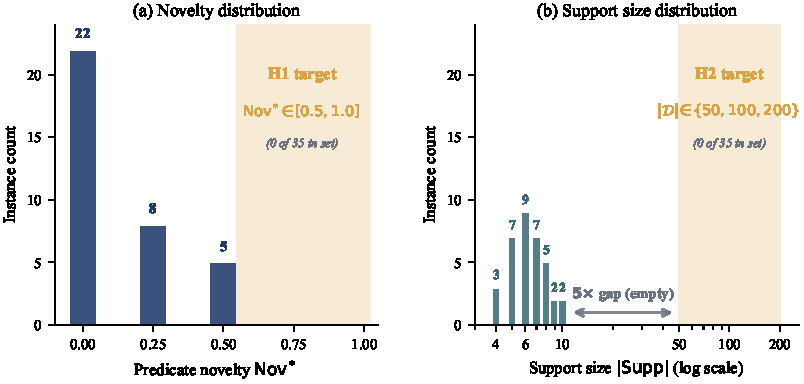
\includegraphics[width=\textwidth]{figures/fig_difficulty.pdf}
\caption{Current Level~3 set vs DeFAb-Hard target regions. (left) Predicate novelty $\Nov^*$ distribution: 63\% of instances have $\Nov^* = 0$ (existing predicates only), 37\% have $\Nov^* > 0$ (max 0.5). H1 target region ($\Nov^* \geq 0.5$) is essentially empty in the current set. (right) Support size distribution: max 10, concentrated at 4--8. H2 target ($|\D| \in \{50, 100, 200\}$, depth $\geq 5$) is far outside the current range. The current set rewards monster-barring; DeFAb-Hard targets lemma-incorporation.}
\label{fig:difficulty}
\end{figure}

The structural difficulty distribution $\sigma(I) = (\ell, |\Supp|, |\Hgold|, \min|h|, \Nov^*)$ for the released Tier~0 Level~3 set: mean $|\Supp| = 6.74$ (std 1.38, range 4--10), mean $\Nov^* = 0.143$ (std 0.226, range 0--0.5), all instances have $|\Hgold| = 1$ and $\min|h| = 1$. The support-size distribution clusters in the 4--10 range far below the DeFAb-Hard H2 targets of 50--200. Figure~\ref{fig:difficulty} visualizes these distributions against pre-registered target regions.


%% =================================================================
\section{M5 Implementation Details}\label{app:m5details}
%% =================================================================

Images for M5 are harvested from three linked knowledge bases. Wikidata's P18 ``image'' property is SPARQL-queryable and provides entity images at configurable resolution (default 640px). VisualSem~\cite{geigle2024babelimagenet} contributes approximately 938{,}000 images across 90{,}000 nodes that bridge WordNet and BabelNet synsets. BabelNet~5.3 contributes 61.4 million images via a REST API. An \texttt{ImageManifest} indexes entity-to-image associations with source-priority selection in the order Wikidata, VisualSem, BabelNet, and the per-theory coverage ratio $c(\D, \mathcal{I}) = |\{e : \mathcal{I}(e) \neq \emptyset\}| / |\mathrm{entities}(\D)|$ controls inclusion via a configurable threshold $\theta$.

The VLM evaluation panel comprises four models. The closed-source tier consists of GPT-5.2-chat and Claude~Sonnet~4.6, accessed via Azure AI Foundry's multimodal content blocks. The open-source tier consists of Qwen2.5-VL-72B-Instruct-AWQ (2$\times$A100, tensor parallel~2) and Qwen2.5-VL-7B-Instruct (1$\times$A100), served via vLLM on CURC Alpine.

A minimal loader looks as follows.
\begin{verbatim}
import json
with open("instances/tier0/level3_instances.json") as f:
    data = json.load(f)
for inst in data["instances"]:
    theory   = inst["theory"]
    target   = inst["target"]
    candidates = inst["candidates"]
\end{verbatim}


%% =================================================================
\section{Complexity Table}\label{app:complexity}
%% =================================================================

\begin{table}[h]
\centering
\small
\caption{Complexity of key pipeline operations. All are polynomial in theory size $|\D|$.}
\label{tab:complexity}
\begin{tabular}{@{}lc@{}}
\toprule
Operation & Complexity \\
\midrule
Defeasible derivation $\D \pPartial q$ & $O(|R| \cdot |F|)$ \\
Gold-standard verification & P \\
Full-theory criticality $\CritStar(\D, q)$ & $O(|\D|^2 \cdot |F|)$ \\
Full pipeline per instance & $O(|\D|^3)$ \\
\bottomrule
\end{tabular}
\end{table}


%% =================================================================
\section{Datasheet for DeFAb}\label{app:datasheet}
%% =================================================================

\subsection*{Motivation}

\begin{itemize}[nosep]
\item \textbf{Purpose:} DeFAb was created to evaluate and train foundation models on defeasible abduction --- the ability to construct hypotheses that explain anomalies by overriding default conclusions while preserving unrelated expectations. No existing benchmark combines formally verifiable gold-standard hypotheses with conservativity constraints, contamination-resistant evaluation, and verifier-backed finetuning signal.
\item \textbf{Creators:} Patrick Cooper, University of Colorado Boulder.
\item \textbf{Funding:} University of Colorado Boulder Department of Computer Science.
\end{itemize}

\subsection*{Composition}

\begin{itemize}[nosep]
\item \textbf{Instance types:} Each instance is an abductive reasoning task: ablated defeasible theory $\Dm$, target literal $q$, candidate hypothesis set $\Hcand$, gold-standard answers $\Hgold$. Level~1: fact completion. Level~2: rule abduction. Level~3: conservative defeater construction.
\item \textbf{Instance count:} Tier~0: 409 (374 L2, 35 L3). Tier~1: 324,511 (182K L1, 142K L2) across five domains. Tier~2: 44,902. Tier~3: 2,580. Tier~RTS: 246+ (100 L1 + 60 L2 + 6 L3 for \texttt{rts\_engagement}, $\sim$80 for \texttt{lux\_ai\_s3}, session-dependent for \texttt{sc2live}). Synthetic: 409 contamination-control instances. \textsc{DeFAb-Hard} (pre-registered, TBD): target 1{,}000+ H1 + 300 H2 + 100 H3 + $\geq 50$ intersection instances. Total (Tiers 0--3 + RTS, excluding pending): 372,648+.
\item \textbf{Rule base:} 33.75 million materialized rules from 18 knowledge sources.
\item \textbf{Sensitive content:} None. All instances derived from formal logic programs over scientific and commonsense knowledge.
\item \textbf{Personal data:} None. No human subjects, no crowdsourcing.
\end{itemize}

\subsection*{Collection Process}

\begin{itemize}[nosep]
\item \textbf{Acquisition:} Generated by a deterministic polynomial-time pipeline from publicly available knowledge bases. 35 high-novelty Level~3 defeaters authored by the paper's author.
\item \textbf{Time frame:} Source knowledge bases span 1984 (Cyc) to 2025 (UMLS 2025AB, YAGO 4.5).
\item \textbf{Ethical review:} No IRB review required (no human subjects). All source KBs publicly available under open licenses.
\end{itemize}

\subsection*{Preprocessing}

\begin{itemize}[nosep]
\item \textbf{Preprocessing:} Source KBs converted to definite logic programs, then to defeasible theories via $\kappa$. Cross-ontology extraction normalizes concept names. Non-English content filtered at extraction.
\item \textbf{Raw data:} All source KBs publicly available (see Section~\ref{sec:conclusion}).
\end{itemize}

\subsection*{Uses}

\begin{itemize}[nosep]
\item \textbf{Intended uses:} Evaluating foundation models on non-monotonic reasoning, belief revision, and grounded hypothesis generation. Training via DPO, RLHF, and GRPO using the polynomial-time verifier as exact reward. Evaluating LLM-as-commander policies under formal ROE constraints (Tier~RTS).
\item \textbf{Not intended for:} Real-world scientific, legal, or medical decisions. The Tier~RTS KBs use StarCraft~II / Lux~AI as proxy environments and do not encode operational ROE.
\end{itemize}

\subsection*{Distribution}

\begin{itemize}[nosep]
\item \textbf{License:} MIT (pipeline and produced instances). Source KB licenses: YAGO (CC-BY 4.0), WordNet (Princeton License), LKIF Core (Apache 2.0), MatOnto (CC-BY 4.0), Wikidata (CC0 1.0), ConceptNet (CC-BY-SA 4.0), Gene Ontology (CC-BY 4.0), UMLS (NLM License), SUMO (GPLv2), FrameNet (CC-BY 3.0).
\item \textbf{Platform:} HuggingFace Datasets (\url{https://huggingface.co/datasets/PatrickAllenCooper/DeFAb}).
\end{itemize}

\subsection*{Maintenance}

\begin{itemize}[nosep]
\item \textbf{Maintainer:} Patrick Cooper, University of Colorado Boulder (\texttt{patrick.cooper@colorado.edu}).
\item \textbf{Duration:} At least 5 years from publication. Generation pipeline enables re-generation from updated source KBs.
\item \textbf{Versioning:} Semantic versioning. Tier~0 instances frozen at v1.0 for cross-study comparability. Additional tiers are additive.
\item \textbf{Issues:} GitHub repository (\url{https://github.com/PatrickAllenCooper/blanc}).
\end{itemize}


\newpage
\section*{NeurIPS Paper Checklist}

\begin{enumerate}

\item {\bf Claims}
    \item[] Answer: \answerYes{}
    \item[] Justification: The introduction lists six numbered contributions, each developed in corresponding sections (Sections~\ref{sec:design}--\ref{sec:finetuning}). All accuracy figures include Wilson 95\% CIs. Claims about dataset scale are backed by Table~\ref{tab:kbsummary}. The symbolic baseline is documented at \texttt{experiments/results/symbolic\_baseline\_l2.json} and \texttt{symbolic\_baseline\_l3.json}.

\item {\bf Limitations}
    \item[] Answer: \answerYes{}
    \item[] Justification: Section~\ref{sec:discussion} discusses limitations: Tier~0 Level~3 sample size (35 instances, easy distribution), M1 decoder approximation, sparse automated Level~3 generation, structural contamination residual, and pending M5/DeFAb-Hard results.

\item {\bf Theory assumptions and proofs}
    \item[] Answer: \answerYes{}
    \item[] Justification: All propositions and theorems are numbered. Proof sketches appear in Appendix~\ref{app:proofs}; full proofs in the companion technical report~\cite{cooper2026defab}. Assumptions stated explicitly (e.g., Proposition~\ref{prop:strict} assumes all-strict partition).

\item {\bf Experimental result reproducibility}
    \item[] Answer: \answerYes{}
    \item[] Justification: Section~\ref{sec:evaluation} specifies all models, decoding parameters (greedy, temperature 0), prompting strategies, and instance generation parameters. Full pipeline and all instances are released.

\item {\bf Open access to data and code}
    \item[] Answer: \answerYes{}
    \item[] Justification: Dataset, pipeline, and harness released under MIT license (Section~\ref{sec:conclusion}). Evaluated models accessible via commercial APIs and open-source hosting.

\item {\bf Experimental setting/details}
    \item[] Answer: \answerYes{}
    \item[] Justification: Section~\ref{subsec:setup} specifies all models, API endpoints, compute resources, and decoding parameters. Section~\ref{sec:design} specifies distractor count ($k = 5$), partition strategies, and the three-stage decoder pipeline.

\item {\bf Experiment statistical significance}
    \item[] Answer: \answerYes{}
    \item[] Justification: Table~\ref{tab:main} reports Wilson 95\% confidence intervals. McNemar's test used for pairwise model comparisons with reported $p$-values.

\item {\bf Experiments compute resources}
    \item[] Answer: \answerYes{}
    \item[] Justification: Section~\ref{subsec:setup} specifies Azure AI Foundry (eastus2, Global Standard) for closed-source models and CURC Alpine (NVIDIA A100 80\,GB) for open-source models.

\item {\bf Code of ethics}
    \item[] Answer: \answerYes{}
    \item[] Justification: All source KBs publicly available under open licenses. No personal data, crowdsourcing, or human subjects involved.

\item {\bf Broader impacts}
    \item[] Answer: \answerYes{}
    \item[] Justification: Positive: improved evaluation of reasoning deficits may accelerate development of more reliable AI. The verifier-backed finetuning substrate supports development of models that satisfy formal conservativity constraints. Negative: low risk; formal logic benchmark with no direct path to harmful deployment.

\item {\bf Safeguards}
    \item[] Answer: \answerNA{}
    \item[] Justification: Released artifacts are evaluation instances from public logic-based KBs and a deterministic pipeline. No pretrained models released; no sensitive content. Tier~RTS KBs use StarCraft~II / Lux~AI as proxy environments, not operational ROE.

\item {\bf Licenses for existing assets}
    \item[] Answer: \answerYes{}
    \item[] Justification: All KBs cited with primary references. License information in Section~\ref{sec:conclusion} and Datasheet (Appendix~\ref{app:datasheet}). All licenses compatible with MIT release of derived instances.

\item {\bf New assets}
    \item[] Answer: \answerYes{}
    \item[] Justification: DeFAb dataset documented via Datasheet (Appendix~\ref{app:datasheet}), released with README, JSON format specification, and Croissant metadata (core and RAI fields). Tier~RTS additions ship with formal certification report at \texttt{data/rts\_certification\_report.json} and verifier-gated commander policy at \texttt{src/blanc/sc2live/policies/commander.py}, all under MIT license.

\item {\bf Crowdsourcing and human subjects}
    \item[] Answer: \answerNA{}
    \item[] Justification: No crowdsourcing or human subjects involved. All instances generated by deterministic pipeline.

\item {\bf IRB approvals}
    \item[] Answer: \answerNA{}
    \item[] Justification: No human subjects involved. IRB review not required.

\item {\bf Declaration of LLM usage}
    \item[] Answer: \answerYes{}
    \item[] Justification: LLMs are the primary evaluated objects (Section~\ref{sec:evaluation}). The D3 semantic parser in the decoder pipeline employs a language model for hypothesis extraction from narrative responses.

\end{enumerate}


\end{document}
